% Template:     Informe/Reporte LaTeX
% Documento:    Archivo principal
% Versión:      4.7.4 (04/04/2018)
% Codificación: UTF-8
%
% Autor: Pablo Pizarro R.
%        Facultad de Ciencias Físicas y Matemáticas
%        Universidad de Chile
%        pablo.pizarro@ing.uchile.cl, ppizarror.com
%
% Manual template: [http://latex.ppizarror.com/Template-Informe/]
% Licencia MIT:    [https://opensource.org/licenses/MIT/]

% CREACIÓN DEL DOCUMENTO
\documentclass[letterpaper,11pt]{article} % Articulo tamaño carta, 11pt
\usepackage[utf8]{inputenc} % Codificación UTF-8

% INFORMACIÓN DEL DOCUMENTO
\def\titulodelinforme {Segmentación basada en grafos}
\def\temaatratar {Algoritmo de Felzenszwalb}

\def\autordeldocumento {Daniel Soto}
\def\nombredelcurso {Procesamiento y Análisis de Imágenes}
\def\codigodelcurso {CC5508}

\def\nombreuniversidad {Universidad de Chile}
\def\nombrefacultad {Facultad de Ciencias Físicas y Matemáticas}
\def\departamentouniversidad {Departamento de Ciencias de la Computación}
\def\imagendepartamento {departamentos/dcc}
\def\imagendepartamentoescala {0.2}
\def\localizacionuniversidad {Santiago, Chile}

% INTEGRANTES, PROFESORES Y FECHAS
\def\tablaintegrantes {
\begin{tabular}{ll}
	Alumno:
		& \begin{tabular}[t]{@{}l@{}}
			Daniel Soto
		\end{tabular} \\
  Profesores:
    & \begin{tabular}[t]{@{}l@{}}
      José M. Saavedra \\
      Mauricio Cerda Villablanca \\
    \end{tabular} \\
  Ayudante:
    & \begin{tabular}[t]{@{}l@{}}
      Andrés Ferrada L. \\
    \end{tabular} \\
	\multicolumn{2}{l}{Fecha de entrega: \today} \\
	\multicolumn{2}{l}{\localizacionuniversidad}
\end{tabular}
}

% CONFIGURACIONES
% Template:     Informe/Reporte LaTeX
% Documento:    Configuraciones del template
% Versión:      4.7.3 (05/02/2018)
% Codificación: UTF-8
%
% Autor: Pablo Pizarro R.
%        Facultad de Ciencias Físicas y Matemáticas
%        Universidad de Chile
%        pablo.pizarro@ing.uchile.cl, ppizarror.com
%
% Manual template: [http://latex.ppizarror.com/Template-Informe/]
% Licencia MIT:    [https://opensource.org/licenses/MIT/]

% CONFIGURACIONES GENERALES
\def\addemptypagetwosides {false} % Añade páginas en blanco al imprimir a 2 caras
\def\columnsepwidth {2.1}         % Separación entre columnas [em]
\def\defaultinterline {1.0}       % Interlineado por defecto [pt]
\def\defaultnewlinesize {11}      % Tamaño del salto de línea [pt]
\def\documentlang {es-CL}         % Define el idioma del documento
\def\fontdocument {lmodern}       % Tipografía (lmodern,arial,helvet)
\def\numberedequation {true}      % Ecuaciones con \insert... numeradas
\def\pointdecimal {false}         % Números decimales con punto en vez de coma
\def\romanpageuppercase {false}   % Páginas en número romano en mayúsculas
\def\showlinenumbers {false}      % Muestra los números de línea del documento
\def\tablepadding {1.0}           % Espaciado de celda de las tablas

% ESTILO PORTADA Y HEADER-FOOTER
\def\hfstyle {style1}             % Estilo del header-footer (8 estilos distintos)
\def\portraitstyle {style1}       % Estilo de la portada (16 estilos distintos)

% MÁRGENES DE PÁGINA
\def\firstpagemargintop {3.8}     % Margen superior página portada [cm]
\def\pagemarginbottom {2.7}       % Margen inferior página [cm]
\def\pagemarginleft {2.54}        % Margen izquierdo página [cm]
\def\pagemarginright {2.54}       % Margen derecho página [cm]
\def\pagemargintop {3.0}          % Margen superior página [cm]

% CONFIGURACIÓN DE LAS LEYENDAS - CAPTION
\def\captionalignment {justified} % Alineado leyenda (justified,centered,left,right)
\def\captionlessmarginimage {0.1} % Margen sup/inf de figuras si no hay leyenda [cm]
\def\captionlrmargin {2.0}        % Márgenes izq/der de la leyenda [cm]
\def\captiontbmarginfigure {9.35} % Margen sup/inf de la leyenda en figuras [pt]
\def\captiontbmargintable {7.0}   % Margen sup/inf de la leyenda en tablas [pt]
\def\captiontextbold {false}      % Etiquetas (Código,Figura,Tabla) en negrita
\def\codecaptiontop {true}        % Leyenda arriba del código fuente
\def\figurecaptiontop {false}     % Leyenda arriba de las imágenes
\def\showsectioncaption {none}    % Número de la sección en objetos (none,sec,ssec,sssec)
\def\tablecaptiontop {true}       % Leyenda arriba de las tablas

% CONFIGURACIÓN DEL ÍNDICE
\def\charafterobjectindex {.}     % Carácter después de número de fig,tabla,código
\def\indexdepth {3}               % Profundidad máxima del índice
\def\indextitlemargin {7.0}       % Margen título en índice \insertindextitle [pt]
\def\showdotpagenumindex {true}   % Muestra puntos entre objeto y número de página
\def\showindex {true}             % Muestra el índice
\def\showindexofcode {true}       % Muestra la lista de códigos fuente
\def\showindexofcontents {true}   % Muestra la lista de contenidos
\def\showindexoffigures {true}    % Muestra la lista de figuras
\def\showindexoftables {true}     % Muestra la lista de tablas

% CONFIGURACIÓN DE LOS COLORES DEL DOCUMENTO
\def\captioncolor {black}         % Color de la etiqueta (Código,Figura,Tabla)
\def\captiontextcolor {black}     % Color de la leyenda
\def\colorpage {white}            % Color de la página
\def\highlightcolor {yellow}      % Color del subrayado con \hl
\def\indextitlecolor {black}      % Color de los títulos del índice
\def\linenumbercolor {dgray}      % Color del número de línea (\showlinenumbers)
\def\linkcolor {black}            % Color de los links del doc.
\def\maintextcolor {black}        % Color principal del texto
\def\numcitecolor {black}         % Color del número de las referencias o citas
\def\portraittitlecolor {black}   % Color de los títulos de la portada
\def\showborderonlinks {false}    % Color de un links por un recuadro de color
\def\subsubtitlecolor {black}     % Color de los sub-subtítulos
\def\subtitlecolor {black}        % Color de los subtítulos
\def\tablelinecolor {black}       % Color de las líneas de las tablas
\def\titlecolor {black}           % Color de los títulos
\def\urlcolor {magenta}           % Color de los enlaces web (\url,\href)

% CONFIGURACIÓN DE FIGURAS
\def\defaultimagefolder {images/} % Carpeta raíz de las imágenes
\def\marginbottomimages {-0.2}    % Margen inferior figura [cm]
\def\marginfloatimages {-13.0}    % Margen sup. figuras \insertimageleft/right [pt]
\def\margintopimages {0.0}        % Margen superior figura [cm]

% ANEXO, CITAS, REFERENCIAS
\def\apaciterefsep {9}            % Separación entre referencias {apacite} [pt]
\def\appendixindepobjnum {true}   % Anexo usa número objetos de forma independiente
\def\bibtexrefsep {9}             % Separación entre referencias {bibtex} [pt]
\def\donumrefsection {false}      % Sección de referencias numerada
\def\natbibrefsep {5}             % Separación entre referencias {natbib} [pt]
\def\sectionappendixlastchar {.}  % Carácter entre n° de la sec. de anexo y título
\def\showappendixsecindex {false} % Título de la sección de anexos en el índice
\def\showappendixsectitle {false} % Título de la sección de anexo en el informe
\def\stylecitereferences {bibtex} % Estilo cita y referencias (bibtex,apacite,natbib)
\def\twocolumnreferences {false}  % Referencias en dos columnas

% CONFIGURACIÓN DE LOS TÍTULOS
\def\anumsecaddtocounter {true}   % Insertar títulos 'anum' incrementa n° de secciones
\def\fontsizesubsubtitle {\large} % Tamaño sub-subtítulos
\def\fontsizesubtitle {\Large}    % Tamaño subtítulos
\def\fontsizetitle {\huge}        % Tamaño títulos
\def\fontsizetitlei {\huge}       % Tamaño títulos en el índice
\def\showdotontitles {true}       % Punto al final del n° de título/sub(sub)título
\def\stylesubsubtitle {\bfseries} % Estilo sub-subtítulos
\def\stylesubtitle {\bfseries}    % Estilo subtítulos
\def\styletitle {\bfseries}       % Estilo títulos
\def\styletitlei {\bfseries}      % Estilo títulos en el índice

% OPCIONES DEL PDF COMPILADO
\def\addindextobookmarks {false}  % Añade el índice a los marcadores del pdf
\def\cfgbookmarksopenlevel {1}    % Nivel de los marcadores en el pdf (1: secciones)
\def\cfgpdfbookmarkopen {true}    % Expande marcadores hasta el nivel configurado
\def\cfgpdfcenterwindow {true}    % Centra la ventana del lector al abrir el pdf
\def\cfgpdfcopyright {}           % Establece el copyright del documento
\def\cfgpdfdisplaydoctitle {true} % Muestra título del informe como título del pdf
\def\cfgpdffitwindow {false}      % Ajusta la ventana del lector al tamaño del pdf
\def\cfgpdfmenubar {true}         % Muestra el menú del lector al abrir el pdf
\def\cfgpdfpagemode {OneColumn}   % Modo de página en lector (OneColumn,SinglePage)
\def\cfgpdfpageview {FitH}        % Ajuste pag (Fit,FitH,FitV,FitR,FitB,FitBH,FitBV)
\def\cfgpdfsecnumbookmarks {true} % Número de la sección en los marcadores del pdf
\def\cfgpdftoolbar {true}         % Muestra la barra de herramientas del lector pdf
\def\cfgshowbookmarkmenu {true}   % Muestra menú de los marcadores al abrir el pdf
\def\pdfcompileversion {7}        % Versión mínima del pdf compilado (1.x)

% NOMBRE DE OBJETOS
\def\nameabstract {Resumen}           % Nombre del resumen-abstract
\def\nameappendixsection {Anexos}     % Nombre de la sección de anexos/apéndices
\def\nameportraitpage {Portada}       % Etiqueta página de la portada
\def\namereferences {Referencias}     % Nombre de la sección de referencias
\def\nomchapter {Capítulo}            % Nombre de los capítulos
\def\nomltappendixsection {Anexo}     % Etiqueta sección en anexo/apéndices
\def\nomltcont {Índice de Contenidos} % Nombre del índice de contenidos
\def\nomltfigure {Lista de Figuras}   % Nombre del índice de la lista de figuras
\def\nomltsrc {Lista de Códigos}      % Nombre del índice de la lista de código
\def\nomlttable {Lista de Tablas}     % Nombre del índice de la lista de tablas
\def\nomltwfigure {Figura}            % Etiqueta leyenda de las figuras
\def\nomltwsrc {Código}               % Etiqueta leyenda del código fuente
\def\nomltwtable {Tabla}              % Etiqueta leyenda de las tablas


% IMPORTACIÓN DE LIBRERÍAS
% Template:     Informe/Reporte LaTeX
% Documento:    Importación de librerías
% Versión:      4.7.3 (05/02/2018)
% Codificación: UTF-8
%
% Autor: Pablo Pizarro R.
%        Facultad de Ciencias Físicas y Matemáticas
%        Universidad de Chile
%        pablo.pizarro@ing.uchile.cl, ppizarror.com
%
% Manual template: [http://latex.ppizarror.com/Template-Informe/]
% Licencia MIT:    [https://opensource.org/licenses/MIT/]

% LIBRERÍAS IMPORTANTES
\usepackage[spanish,es-nosectiondot,es-lcroman]{babel} % Idioma
\usepackage[T1]{fontenc} % Caracteres acentuados
\usepackage{\fontdocument} % Tipografía del documento
\usepackage{ifthen} % Manejo de condicionales
\ifthenelse{\equal{\showlinenumbers}{true}}{ % Muestra los números de línea
	\usepackage[switch,columnwise,running]{lineno}}{
}

% LIBRERÍAS INDEPENDIENTES
\usepackage{amsmath}       % Librerías matemáticas
\usepackage{amssymb}       % Librerías matemáticas
\usepackage{array}         % Nuevas características a las tablas
\usepackage{bigstrut}      % Líneas horizontales en tablas
\usepackage{bm}            % Caracteres en negrita en ecuaciones
\usepackage{booktabs}      % Permite manejar elementos visuales en tablas
\usepackage{caption}       % Leyendas
\usepackage{changepage}    % Condicionales para administrar páginas
\usepackage{chngcntr}      % Añade números a las leyendas
\usepackage{color}         % Colores
\usepackage{colortbl}      % Administración de color en las tablas
\usepackage{csquotes}      % Citas y comillas
\usepackage{datetime}      % Fechas
\usepackage{floatpag}      % Maneja números de páginas
\usepackage{floatrow}      % Permite adminisrar posiciones en los caption
\usepackage{framed}        % Permite creación de recuadros
\usepackage{gensymb}       % Simbología común
\usepackage{geometry}      % Dimensiones y geometría del documento
\usepackage{graphicx}      % Propiedades extra para los gráficos
\usepackage{lipsum}        % Permite crear párrafos de prueba
\usepackage{listings}      % Permite añadir código fuente
\usepackage{longtable}     % Permite utilizar tablas en varias hojas
\usepackage{lscape}        % Modo página horizontal de página
\usepackage{mathtools}     % Permite utilizar notaciones matemáticas
\usepackage{multicol}      % Múltiples columnas
\usepackage{needspace}     % Maneja los espacios en página
\usepackage{notoccite}     % Desactiva las citas en el índice
\usepackage{pdfpages}      % Permite administrar páginas en pdf
\usepackage{physics}       % Paquete de matemáticas
\usepackage{rotating}      % Permite rotación de objetos
\usepackage{sectsty}       % Cambia el estilo de los títulos
\usepackage{selinput}      % Compatibilidad con acentos
\usepackage{setspace}      % Cambia el espacio entre líneas
\usepackage{siunitx}       % Unidades del sistema internacional
\usepackage{soul}          % Permite subrayar texto
\usepackage{subfig}        % Permite agrupar imágenes
\usepackage{textcomp}      % Simbología común
\usepackage{url}           % Permite añadir enlaces
\usepackage{wasysym}       % Contiene caracteres misceláneos
\usepackage{wrapfig}       % Permite comprimir imágenes
\usepackage{xspace}        % Adminsitra espacios en párrafos y líneas

% LIBRERÍAS CON PARÁMETROS
\usepackage[makeroom]{cancel} % Cancelar términos en fórmulas
\usepackage[inline]{enumitem} % Permite enumerar ítems
\usepackage[bottom,norule,hang]{footmisc} % Estilo pie de página
\usepackage[subfigure,titles]{tocloft} % Maneja entradas en el índice
\usepackage[pdfencoding=auto,psdextra]{hyperref} % Enlaces, referencias
\usepackage[figure,table,lstlisting]{totalcount} % Contador de objetos
\usepackage[normalem]{ulem} % Permite tachar y subrayar
\usepackage[usenames,dvipsnames]{xcolor} % Paquete de colores avanzado

% LIBRERÍAS CONDICIONALES
\ifthenelse{\equal{\showdotontitles}{true}}{ % Agrega puntos a los títulos/subtítulos
	\usepackage{secdot}
	\sectiondot{subsection}
	\sectiondot{subsubsection}}{
}
\ifthenelse{\equal{\stylecitereferences}{natbib}}{ % Formato citas natbib
	\usepackage{natbib}
}{
	\ifthenelse{\equal{\stylecitereferences}{apacite}}{ % Formato citas apacite
		\usepackage{apacite}
	}{
		\ifthenelse{\equal{\stylecitereferences}{bibtex}}{ % Formato citas bibtex
		}{
		}
	}
}
\ifthenelse{\equal{\showappendixsecindex}{true}}{ % Anexos/Apéndices
	\usepackage[toc]{appendix}
}{
	\usepackage{appendix}
}

% LIBRERÍAS DEPENDIENTES
\usepackage{bookmark}      % Administración de marcadores en pdf
\usepackage{fancyhdr}      % Encabezados y pie de páginas
\usepackage{float}         % Administrador de posiciones de objetos
\usepackage{hyperxmp}      % Etiquetas opcionales para el pdf compilado
\usepackage{multirow}      % Agrega nuevas opciones a las tablas
\usepackage{titlesec}      % Administración de títulos


% IMPORTACIÓN DE FUNCIONES
% Template:     Informe/Reporte LaTeX
% Documento:    Funciones del núcleo del template
% Versión:      4.7.3 (05/02/2018)
% Codificación: UTF-8
%
% Autor: Pablo Pizarro R.
%        Facultad de Ciencias Físicas y Matemáticas
%        Universidad de Chile
%        pablo.pizarro@ing.uchile.cl, ppizarror.com
%
% Manual template: [http://latex.ppizarror.com/Template-Informe/]
% Licencia MIT:    [https://opensource.org/licenses/MIT/]

\newcommand{\throwerror}[2]{
	% Lanza un mensaje de error
	% 	#1	Función del error
	%	#2	Mensaje
	\errmessage{LaTeX Error: \noexpand#1 #2 (linea \the\inputlineno)}
	\stop
}

\newcommand{\throwwarning}[1]{
	% Lanza un mensaje de advertencia
	%	#1	Mensaje
	\errmessage{LaTeX Warning: #1 (linea \the\inputlineno)}
}

\newcommand{\throwbadconfig}[3]{
	% Lanza un mensaje de error indicando mala configuración
	%	#1	Mensaje de error
	% 	#2	Configuración usada
	%	#3	Valores esperados
	\errmessage{LaTeX Warning: #1 \noexpand #2=#2. Valores esperados: #3}
	\stop
}

\newcommand{\throwbadconfigondoc}[3]{
	% Lanza un mensaje de error indicando mala configuración dentro de begin{document}
	%	#1	Mensaje de error
	% 	#2	Configuración usada
	%	#3	Valores esperados
	\errmessage{#1 \noexpand #2=#2. Valores esperados: #3}
	\stop
}

\newcommand{\checkvardefined}[1]{
	% Comprueba si una variable está definida
	%	#1	Variable
	\ifthenelse{\isundefined{#1}}{
		\errmessage{LaTeX Warning: Variable \noexpand#1 no definida}
		\stop
	}{}
}

\newcommand{\checkextravarexist}[2]{
	% Comprueba si una variable está definida
	%	#1	Variable
	%	#2	Mensaje
	\ifthenelse{\isundefined{#1}}{
		\errmessage{LaTeX Warning: Variable \noexpand#1 no definida}
		\ifx\hfuzz#2\hfuzz
			\errmessage{LaTeX Warning: Defina la variable en el bloque de INFORMACION DEL DOCUMENTO al comienzo del archivo principal del Template}
		\else
			\errmessage{LaTeX Warning: #2}
		\fi
	}{}
}

\newcommand{\emptyvarerr}[3]{
	% Lanza un mensaje de error si una variable no ha sido definida
	% 	#1	Función del error
	%	#2	Variable
	%	#3	Mensaje
	\ifx\hfuzz#2\hfuzz
		\errmessage{LaTeX Warning: \noexpand#1 #3 (linea \the\inputlineno)}
	\fi
}

\newcommand{\setcaptionmargincm}[1]{
	% Cambiar el margen de los caption
	% 	#1	Margen en centímetros
	\captionsetup{margin=#1cm}
}

\newcommand{\setpagemargincm}[4]{
	% Cambia márgenes de las páginas [cm]
	% 	#1	Margen izquierdo
	%	#2	Margen superior
	%	#3	Margen derecho
	%	#4	Margen inferior
	\newgeometry{left=#1cm, top=#2cm, right=#3cm, bottom=#4cm}
}

\newcommand{\changemargin}[2]{
	% Cambia los márgenes del documento
	%	#1 Margen izquierdo
	%	#2 Margen derecho
	\emptyvarerr{\changemargin}{#1}{Margen izquierdo no definido}
	\emptyvarerr{\changemargin}{#2}{Margen derecho no definido}
	\list{}{\rightmargin#2\leftmargin#1}\item[]
}
\let\endchangemargin=\endlist

\newcommand{\bgtemplatetestimg}{
	% Imagen de prueba tikz
	\definecolor{c040302}{RGB}{4, 3, 2}
	\definecolor{cb26929}{RGB}{178,105, 41}
	\definecolor{cfa943c}{RGB}{250, 148, 60}
	\definecolor{cfdc594}{RGB}{253, 197, 148}
	\begin{tikzpicture}[y=1.0pt, x=1.0pt, yscale=-1, xscale=1, inner sep=0pt, outer sep=0pt, opacity=0.1]
	\path[fill=cfdc594](46.3187,318.2550)..controls(46.0737,317.5650)and
	(45.7487,314.0750)..(45.5987,310.5)--(45.3247,304)--(37.8247,303.5)--(30.3247,303)--(29.8247,295.5)-- (29.3247,288)--(21.8247,287.5)--(14.3247,287)--(13.8247,271.5)--(13.3247,256)--(5.8247,255.5)-- (-1.6753,255)--(-1.6753,206.5)--(-1.6753,158)--(5.8247,157.5)--(13.3247,157)--(13.8247,141.5)-- (14.3247,126)--(21.8247,125.5)--(29.3247,125)--(29.8247,109.5)--(30.3247,94)--(37.8247,93.5)-- (45.3247,93)--(45.8247,69.5)--(46.3247,46)--(53.8247,45.5)--(61.3247,45)--(61.8247,29.5)-- (62.3247,14)--(69.8247,13.5)--(77.3247,13)--(77.8247,5.5)--(78.3247,-2)--(94.8247,-2)-- (111.3247,-2)--(111.8247,5.5)--(112.3247,13)--(119.8247,13.5)--(127.3247,14)--(127.8247,21.5)-- (128.3247,29)--(166.8247,29)--(205.3247,29)--(205.8247,21.5)--(206.3247,14)--(213.8247,13.5)-- (221.3247,13)--(221.8247,5.5)--(222.3247,-2)--(230.8247,-2)--(239.3247,-2)--(239.8247,5.5)-- (240.3247,13)--(247.8247,13.5)--(255.3247,14)--(255.8247,21.5)--(256.3247,29)--(263.8247,29.5)-- (271.3247,30)--(271.8247,45.5)--(272.3247,61)--(279.8247,61.5)--(287.3247,62)--(287.8247,85.5)-- (288.3247,109)--(295.8247,109.5)--(303.3247,110)--(303.8247,133.5)--(304.3247,157)--(311.8247,157.5)-- (319.3247,158)--(319.3247,198.5)--(319.3247,239)--(311.8247,239.5)--(304.3247,240)--(303.8247,255.5)-- (303.3247,271)--(295.8247,271.5)--(288.3247,272)--(287.8247,279.5)--(287.3247,287)--(279.8247,287.5)-- (272.3247,288)--(271.8247,295.5)--(271.3247,303)--(263.8247,303.5)--(256.3247,304)--(255.8247,311.5)-- (255.3247,319)--(151.0447,319.2550)..controls(68.1357,319.4570)and (46.6737,319.2530)..(46.3187,318.2550)--cycle(173.8247,142.5)-- (173.8247,127.5)--(166.8247,127.5)--(159.8247,127.5)-- (159.8247,142.5)--(159.8247,157.5)--(166.8247,157.5)-- (173.8247,157.5)--cycle(269.8247,126.5)--(269.8247,111.5)-- (262.8247,111.5)--(255.8247,111.5)--(255.8247,126.5)-- (255.8247,141.5)--(262.8247,141.5)--(269.8247,141.5)--cycle; \path[fill=cfa943c](47.3187,317.2550)..controls(47.0737,316.5650)and (46.7487,313.0750)..(46.5987,309.5)--(46.3247,303)--(38.8247,302.5)--(31.3247,302)--(30.8247,294.5)-- (30.3247,287)--(22.8247,286.5)--(15.3247,286)--(14.8247,270.5)--(14.3247,255)--(6.8247,254.5)-- (-0.6753,254)--(-0.6753,206.5)--(-0.6753,159)--(6.8247,158.5)--(14.3247,158)--(14.8247,142.5)-- (15.3247,127)--(22.8247,126.5)--(30.3247,126)--(30.8247,110.5)--(31.3247,95)--(38.8247,94.5)-- (46.3247,94)--(46.8247,70.5)--(47.3247,47)--(54.8247,46.5)--(62.3247,46)--(62.8247,30.5)-- (63.3247,15)--(70.8247,14.5)--(78.3247,14)--(78.8247,6.5)--(79.3247,-1)--(94.8247,-1)-- (110.3247,-1)--(110.8247,6.5)--(111.3247,14)--(118.8247,14.5)--(126.3247,15)--(126.8247,22.5)-- (127.3247,30)--(166.8247,30)--(206.3247,30)--(206.8247,22.5)--(207.3247,15)--(214.8247,14.5)-- (222.3247,14)--(222.8247,6.5)--(223.3247,-1)--(230.8247,-1)--(238.3247,-1)--(238.8247,6.5)-- (239.3247,14)--(246.8247,14.5)--(254.3247,15)--(254.8247,22.5)--(255.3247,30)--(262.8247,30.5)-- (270.3247,31)--(270.8247,46.5)--(271.3247,62)--(278.8247,62.5)--(286.3247,63)--(286.8247,86.5)-- (287.3247,110)--(294.8247,110.5)--(302.3247,111)--(302.8247,134.5)--(303.3247,158)--(310.8247,158.5)-- (318.3247,159)--(318.3247,198.5)--(318.3247,238)--(310.8247,238.5)--(303.3247,239)--(302.8247,254.5)-- (302.3247,270)--(294.8247,270.5)--(287.3247,271)--(286.8247,278.5)--(286.3247,286)--(278.8247,286.5)-- (271.3247,287)--(270.8247,294.5)--(270.3247,302)--(262.8247,302.5)--(255.3247,303)--(254.8247,310.5)-- (254.3247,318)--(151.0447,318.2550)..controls(68.9357,318.4570)and (47.6737,318.2520)..(47.3187,317.2550)--cycle(253.8247,294.70).. controls(253.8247,290.7440)and(254.3267,287.3980)..(255.0247,286.70).. controls(255.7227,286.0020)and(259.0687,285.5)..(263.0247,285.5)-- (269.8247,285.5)--(269.8247,278.70)..controls(269.8247,274.7440)and (270.3267,271.3980)..(271.0247,270.70)..controls(271.7227,270.0020)and (275.0687,269.5)..(279.0247,269.5)--(285.8247,269.5)-- (285.8247,254.70)..controls(285.8247,244.5220)and(286.1997,239.5250).. (287.0247,238.70)..controls(287.7227,238.0020)and(291.0687,237.5).. (295.0247,237.5)--(301.8247,237.5)--(301.8247,206)-- (301.8247,174.5)--(294.8247,174.5)--(287.8247,174.5)-- (287.8247,189.80)..controls(287.8247,200.3670)and(287.4537,205.4710).. (286.6247,206.30)..controls(285.9267,206.9980)and(282.5807,207.5).. (278.6247,207.5)--(271.8247,207.5)--(271.8247,214.30)..controls (271.8247,218.2560)and(271.3227,221.6020)..(270.6247,222.30)..controls (269.9267,222.9980)and(266.5807,223.5)..(262.6247,223.5)-- (255.8247,223.5)--(255.8247,230.3780)..controls(255.8247,234.9380)and (255.3687,237.6340)..(254.4727,238.3780)..controls(252.4847,240.0280)and (176.6787,239.9540)..(175.0247,238.30)..controls(174.3337,237.6090)and (173.8247,234.30)..(173.8247,230.5)..controls(173.8247,226.70)and (174.3337,223.3910)..(175.0247,222.70)..controls(175.9167,221.8080)and (186.1807,221.5)..(215.0247,221.5)--(253.8247,221.5)-- (253.8247,214.5)--(253.8247,207.5)--(249.0747,207.3720)..controls (246.4627,207.3020)and(235.9997,206.9640)..(225.8247,206.6220)-- (207.3247,206)--(206.8247,198.5)--(206.3247,191)--(190.8247,190.5)--(175.3247,190)--(174.8247,182.5)-- (174.3247,175)--(134.8247,175)--(95.3247,175)--(94.8247,182.5)--(94.3247,190)--(86.8247,190.5)-- (79.3247,191)--(79.3247,222.5)--(79.3247,254)--(86.8247,254.5)--(94.3247,255)--(94.8247,270.5)-- (95.3247,286)--(102.8247,286.5)--(110.3247,287)-- (110.6187,294.2500)--(110.9127,301.5)--(182.3687,301.5)-- (253.8247,301.5)--cycle(174.6247,158.30)..controls (176.4747,156.4500)and(176.2867,128.1290)..(174.4147,126.5750)..controls (173.5527,125.8600)and(170.3467,125.5210)..(166.1647,125.7030)-- (159.3247,126)--(159.0477,141.4580)..controls(158.8957,149.9600)and (158.9937,157.4970)..(159.2667,158.2080)..controls(159.9187,159.9070)and (172.9397,159.9850)..(174.6257,158.30)--cycle(270.6247,142.30).. controls(272.4747,140.4500)and(272.2867,112.1290)..(270.4147,110.5750).. controls(269.5527,109.8600)and(266.3467,109.5210)..(262.1647,109.7030)-- (255.3247,110)--(255.0477,125.4580)..controls(254.8957,133.9600)and (254.9937,141.4970)..(255.2667,142.2080)..controls(255.9187,143.9070)and (268.9397,143.9850)..(270.6257,142.30)--cycle(78.8247,86.5)-- (79.3247,79)--(86.8247,78.5)--(94.3247,78)--(94.8247,70.5)--(95.3247,63)--(102.8247,62.5)-- (110.3247,62)--(110.8247,54.5)--(111.3247,47)-- (118.5747,46.7060)--(125.8247,46.4120)--(125.8247,38.9560)-- (125.8247,31.5)--(119.0247,31.5)..controls(115.0687,31.5)and (111.7227,30.9980)..(111.0247,30.30)..controls(110.3267,29.6020)and (109.8247,26.2560)..(109.8247,22.30)--(109.8247,15.5)-- (94.8247,15.5)--(79.8247,15.5)--(79.8247,30.30)..controls (79.8247,40.4780)and(79.4497,45.4750)..(78.6247,46.30)..controls (77.9267,46.9980)and(74.5807,47.5)..(70.6247,47.5)-- (63.8247,47.5)--(63.8247,71.0440)--(63.8247,94.5880)-- (71.0747,94.2940)--(78.3247,94)--cycle(253.8247,39)-- (253.8247,31.5)--(247.0247,31.5)..controls(243.0687,31.5)and (239.7227,30.9980)..(239.0247,30.30)..controls(238.3267,29.6020)and (237.8247,26.2560)..(237.8247,22.30)--(237.8247,15.5)-- (230.8247,15.5)--(223.8247,15.5)--(223.8247,22.30)..controls (223.8247,26.2560)and(223.3227,29.6020)..(222.6247,30.30)..controls (221.9267,30.9980)and(218.5807,31.5)..(214.6247,31.5)-- (207.8247,31.5)--(207.8247,39)--(207.8247,46.5)-- (230.8247,46.5)--(253.8247,46.5)--cycle; \path[fill=cb26929](47.3187,317.2550)..controls(47.0737,316.5650)and (46.7487,313.0750)..(46.5987,309.5)--(46.3247,303)--(38.8247,302.5)--(31.3247,302)--(30.8247,294.5)-- (30.3247,287)--(22.8247,286.5)--(15.3247,286)--(14.8247,270.5)--(14.3247,255)--(6.8247,254.5)-- (-0.6753,254)--(-0.6753,206.5)--(-0.6753,159)--(6.8247,158.5)--(14.3247,158)--(14.8247,142.5)-- (15.3247,127)--(22.8247,126.5)--(30.3247,126)--(30.8247,110.5)--(31.3247,95)--(38.8247,94.5)-- (46.3247,94)--(46.8247,70.5)--(47.3247,47)--(54.8247,46.5)--(62.3247,46)--(62.8247,30.5)-- (63.3247,15)--(70.8247,14.5)--(78.3247,14)--(78.8247,6.5)--(79.3247,-1)--(94.8247,-1)-- (110.3247,-1)--(110.8247,6.5)--(111.3247,14)--(118.8247,14.5)--(126.3247,15)--(126.8247,22.5)-- (127.3247,30)--(166.8247,30)--(206.3247,30)--(206.8247,22.5)--(207.3247,15)--(214.8247,14.5)-- (222.3247,14)--(222.8247,6.5)--(223.3247,-1)--(230.8247,-1)--(238.3247,-1)--(238.8247,6.5)-- (239.3247,14)--(246.8247,14.5)--(254.3247,15)--(254.8247,22.5)--(255.3247,30)--(262.8247,30.5)-- (270.3247,31)--(270.8247,46.5)--(271.3247,62)--(278.8247,62.5)--(286.3247,63)--(286.8247,86.5)-- (287.3247,110)--(294.8247,110.5)--(302.3247,111)--(302.8247,134.5)--(303.3247,158)--(310.8247,158.5)-- (318.3247,159)--(318.3247,198.5)--(318.3247,238)--(310.8247,238.5)--(303.3247,239)--(302.8247,254.5)-- (302.3247,270)--(294.8247,270.5)--(287.3247,271)--(286.8247,278.5)--(286.3247,286)--(278.8247,286.5)-- (271.3247,287)--(270.8247,294.5)--(270.3247,302)--(262.8247,302.5)--(255.3247,303)--(254.8247,310.5)-- (254.3247,318)--(151.0447,318.2550)..controls(68.9357,318.4570)and (47.6737,318.2520)..(47.3187,317.2550)--cycle(253.8247,294.70).. controls(253.8247,290.7440)and(254.3267,287.3980)..(255.0247,286.70).. controls(255.7227,286.0020)and(259.0687,285.5)..(263.0247,285.5)-- (269.8247,285.5)--(269.8247,278.70)..controls(269.8247,274.7440)and (270.3267,271.3980)..(271.0247,270.70)..controls(271.7227,270.0020)and (275.0687,269.5)..(279.0247,269.5)--(285.8247,269.5)-- (285.8247,254.70)..controls(285.8247,244.5220)and(286.1997,239.5250).. (287.0247,238.70)..controls(287.7227,238.0020)and(291.0717,237.5).. (295.0367,237.5)--(301.8487,237.5)--(301.5867,198.7500)-- (301.3247,160)--(294.8247,160)--(288.3247,160)-- (288.0547,182.4210)..controls(287.8807,196.9060)and(287.3947,205.3120).. (286.6827,206.1710)..controls(285.9607,207.0410)and(283.2017,207.5).. (278.7027,207.5)--(271.8247,207.5)--(271.8247,214.30)..controls (271.8247,218.2560)and(271.3227,221.6020)..(270.6247,222.30)..controls (269.9267,222.9980)and(266.5807,223.5)..(262.6247,223.5)-- (255.8247,223.5)--(255.8247,230.3780)..controls(255.8247,234.9380)and (255.3687,237.6340)..(254.4727,238.3780)..controls(252.4847,240.0280)and (176.6787,239.9540)..(175.0247,238.30)..controls(174.3337,237.6090)and (173.8247,234.30)..(173.8247,230.5)..controls(173.8247,226.70)and (174.3337,223.3910)..(175.0247,222.70)..controls(175.9167,221.8080)and (186.1807,221.5)..(215.0247,221.5)--(253.8247,221.5)-- (253.8247,214.5)--(253.8247,207.5)--(247.0747,207.4850)..controls (243.3627,207.4770)and(239.7747,207.1200)..(239.1027,206.6930)..controls (238.2507,206.1520)and(237.7967,201.3880)..(237.6027,190.9580)-- (237.3247,176)--(229.8247,175.5)--(222.3247,175)--(222.3247,166.5)--(222.3247,158)--(253.8247,157.5)-- (285.3247,157)--(285.3247,134.5)--(285.3247,112)--(277.8247,111.5)--(270.3247,111)--(269.8247,87.5)-- (269.3247,64)--(261.8247,63.5)--(254.3247,63)-- (254.0497,47.2500)--(253.7737,31.5)--(246.9987,31.5)..controls (243.0637,31.5)and(239.7217,30.9970)..(239.0247,30.30)..controls (238.3267,29.6020)and(237.8247,26.2560)..(237.8247,22.30)-- (237.8247,15.5)--(230.8247,15.5)--(223.8247,15.5)-- (223.8247,22.30)..controls(223.8247,26.2560)and(223.3227,29.6020).. (222.6247,30.30)..controls(221.9277,30.9970)and(218.5897,31.5).. (214.6667,31.5)--(207.9087,31.5)--(207.6167,39.2500)-- (207.3247,47)--(166.8247,47)--(126.3247,47)-- (126.0327,39.2500)--(125.7407,31.5)--(118.9827,31.5)..controls (115.0597,31.5)and(111.7217,30.9970)..(111.0247,30.30)..controls (110.3267,29.6020)and(109.8247,26.2560)..(109.8247,22.30)-- (109.8247,15.5)--(94.8247,15.5)--(79.8247,15.5)-- (79.8247,30.30)..controls(79.8247,40.4780)and(79.4497,45.4750).. (78.6247,46.30)..controls(77.9277,46.9970)and(74.5847,47.5).. (70.6427,47.5)--(63.8607,47.5)--(63.5927,71.2500)-- (63.3247,95)--(55.8247,95.5)--(48.3247,96)--(47.8247,111.5)--(47.3247,127)--(39.8247,127.5)-- (32.3247,128)--(31.8247,143.5)--(31.3247,159)--(23.8247,159.5)--(16.3247,160)--(16.3247,175)-- (16.3247,190)--(23.3247,190.5)--(30.3247,191)--(30.8247,198.5)--(31.3247,206)--(38.8247,206.5)-- (46.3247,207)--(46.8247,214.5)--(47.3247,222)--(62.8247,222.5)--(78.3247,223)--(78.8247,238.5)-- (79.3247,254)--(86.8247,254.5)--(94.3247,255)--(94.8247,270.5)--(95.3247,286)--(102.8247,286.5)-- (110.3247,287)--(110.6187,294.2500)--(110.9127,301.5)-- (182.3687,301.5)--(253.8247,301.5)--cycle(126.2657,158.2080).. controls(125.9927,157.4970)and(125.8947,149.9600)..(126.0467,141.4580)-- (126.3247,126)--(142.5747,125.7250)--(158.8247,125.4500)-- (158.8247,142.4750)--(158.8247,159.5)--(142.7937,159.5)..controls (130.6137,159.5)and(126.6437,159.1900)..(126.2667,158.2080)-- cycle(222.2657,142.2080)..controls(221.9927,141.4970)and (221.8947,133.9600)..(222.0467,125.4580)--(222.3247,110)-- (238.5747,109.7250)--(254.8247,109.4500)--(254.8247,126.4750)-- (254.8247,143.5)--(238.7937,143.5)..controls(226.6137,143.5)and (222.6437,143.1900)..(222.2667,142.2080)--cycle; \path[fill=c040302](46.3247,303)--(79.0747,303.0080)..controls (95.9877,303.0120)and(142.2457,303.1250)..(181.8707,303.2580)-- (253.9167,303.5)--(253.6207,310.2500)--(253.3247,317)-- (151.0447,317.2550)..controls(65.3137,317.4680)and(48.6807,317.2880).. (48.2407,316.1430)..controls(46.9629,307.2110)and(46.3247,303).. (46.3247,303)--cycle(32.2567,300.1840)..controls(31.9597,299.4100) and(31.8537,296.1260)..(32.0207,292.8880)--(32.3247,287)-- (39.3247,287)--(46.3247,287)--(46.3247,294)-- (46.3247,301)--(39.5607,301.2960)..controls(34.4617,301.5190)and (32.6637,301.2460)..(32.2567,300.1840)--cycle(255.8247,294.5460)-- (255.8247,287.5)--(262.8707,287.5)--(269.9167,287.5)-- (269.6207,294.2500)--(269.3247,301)--(262.5747,301.2960)-- (255.8247,301.5920)--cycle(16.2817,284.2480)..controls(15.9977,283.5090) and(15.8917,276.6260)..(16.0457,268.9520)--(16.3247,255)-- (23.3247,255)--(30.3247,255)--(30.3247,270)-- (30.3247,285)--(23.5607,285.2960)..controls(18.6047,285.5130)and (16.6587,285.2330)..(16.2807,284.2480)--cycle(271.8247,278.5460)-- (271.8247,271.5)--(278.8707,271.5)--(285.9167,271.5)-- (285.6207,278.2500)--(285.3247,285)--(278.5747,285.2960)-- (271.8247,285.5920)--cycle(287.8247,254.5460)--(287.8247,239.5)-- (294.8517,239.5)--(301.8787,239.5)--(301.6017,254.2500)-- (301.3247,269)--(294.5747,269.2960)--(287.8247,269.5920)-- cycle(0.3007,252.2960)..controls(0.0267,251.5830)and(-0.0793,230.5250).. (0.0637,205.5)--(0.3247,160)--(6.9587,159.7070)-- (13.5927,159.4140)--(14.2807,190.7070)..controls(14.6597,207.9180)and (14.8247,228.9750)..(14.6467,237.5)--(14.3247,253)-- (7.5607,253.2960)..controls(2.7217,253.5080)and(0.6557,253.2230).. (0.2997,252.2960)--cycle(175.8247,230.5)--(175.8247,223.5)-- (214.8247,223.5)--(253.8247,223.5)--(253.8247,230.5)-- (253.8247,237.5)--(214.8247,237.5)--(175.8247,237.5)-- cycle(303.8247,198.5)--(303.8247,159.4090)--(310.5747,159.7050)-- (317.3247,160.0010)--(317.3247,198.5010)--(317.3247,237.0010)-- (310.5747,237.2970)--(303.8247,237.5930)--cycle(255.8247,214.70).. controls(255.8247,210.7440)and(255.3227,207.3980)..(254.6247,206.70).. controls(253.9267,206.0020)and(250.5807,205.5)..(246.6247,205.5)-- (239.8247,205.5)--(239.8247,190.70)..controls(239.8247,180.5220)and (239.4497,175.5250)..(238.6247,174.70)..controls(237.9267,174.0020)and (234.5807,173.5)..(230.6247,173.5)--(223.8247,173.5)-- (223.8247,166.5)--(223.8247,159.5)--(254.8247,159.5)-- (285.8247,159.5)--(285.8247,182.5)--(285.8247,205.5)-- (279.0247,205.5)..controls(275.0687,205.5)and(271.7227,206.0020).. (271.0247,206.70)..controls(270.3267,207.3980)and(269.8247,210.7440).. (269.8247,214.70)--(269.8247,221.5)--(262.8247,221.5)-- (255.8247,221.5)--cycle(16.0477,142.7500)--(16.3247,128)-- (23.0747,127.7040)--(29.8247,127.4090)--(29.8247,142.4540)-- (29.8247,157.5)--(22.7977,157.5)--(15.7717,157.5)-- cycle(127.8247,142.5)--(127.8247,127.5)--(142.8247,127.5)-- (157.8247,127.5)--(157.8247,142.5)--(157.8247,157.5)-- (142.8247,157.5)--(127.8247,157.5)--cycle(287.8247,134.4540)-- (287.8247,111.4080)--(294.5747,111.7040)--(301.3247,112)-- (301.5937,134.7500)--(301.8627,157.5)--(294.8437,157.5)-- (287.8247,157.5)--cycle(223.8247,126.5)--(223.8247,111.5)-- (238.8247,111.5)--(253.8247,111.5)--(253.8247,126.5)-- (253.8247,141.5)--(238.8247,141.5)--(223.8247,141.5)-- cycle(32.0477,110.7500)--(32.3247,96)--(39.0747,95.7040)-- (45.8247,95.4090)--(45.8247,110.4540)--(45.8247,125.5)-- (38.7977,125.5)--(31.7717,125.5)--cycle(271.8247,86.4540)-- (271.8247,63.4090)--(278.5747,63.7050)--(285.3247,64.0010)-- (285.5937,86.7510)--(285.8627,109.5010)--(278.8437,109.5010)-- (271.8247,109.5010)--cycle(48.0557,70.7500)--(48.3247,48)-- (55.0747,47.7040)--(61.8247,47.4090)--(61.8247,70.4540)-- (61.8247,93.5)--(54.8057,93.5)--(47.7867,93.5)-- cycle(255.8247,46.4540)--(255.8247,31.4090)--(262.5747,31.7050)-- (269.3247,32.0010)--(269.6017,46.7510)--(269.8787,61.5010)-- (262.8517,61.5010)--(255.8247,61.5010)--cycle(64.0477,30.7500)-- (64.3247,16)--(71.0747,15.7040)--(77.8247,15.4090)--(77.8247,30.4540)--(77.8247,45.5)--(70.7977,45.5)-- (63.7707,45.5)--cycle(127.8247,38.5)--(127.8247,31.5)--(166.8247,31.5)--(205.8247,31.5)--(205.8247,38.5)-- (205.8247,45.5)--(166.8247,45.5)--(127.8247,45.5)-- cycle(111.8247,22.4540)--(111.8247,15.4080)--(118.5747,15.7040)-- (125.3247,16)--(125.6207,22.7500)--(125.9167,29.5)-- (118.8707,29.5)--(111.8247,29.5)--cycle(208.0287,22.7500)-- (208.3247,16)--(215.0747,15.7040)--(221.8247,15.4090)-- (221.8247,22.4540)--(221.8247,29.5)--(214.7787,29.5)-- (207.7327,29.5)--cycle(239.8247,22.4540)--(239.8247,15.4080)-- (246.5747,15.7040)--(253.3247,16)--(253.6207,22.7500)-- (253.9167,29.5)--(246.8707,29.5)--(239.8247,29.5)--cycle(80.0287,6.7500)--(80.3247,0)--(94.8247,0)-- (109.3247,0)--(109.6207,6.7500)--(109.9167,13.5)--(94.8247,13.5)--(79.7337,13.5)--cycle(224.0287,6.7500)-- (224.3247,0)--(230.8247,0)--(237.3247,0)--(237.6207,6.7500)--(237.9167,13.5)--(230.8247,13.5)-- (223.7337,13.5)--cycle;
	\end{tikzpicture}
}
\def\bgtemplatetestcode {d0g3}

\newcommand{\importtikzlib}{
	% Se importa la librería tikz
	\usepackage{tikz}
}

\def\beginplandscape {
	% Inicia el modo de página horizontal
	\newgeometry{landscape,left=\pagemarginleft cm,top=\pagemargintop cm,right=\pagemarginright cm,bottom=\pagemarginbottom cm}
	\headwidth=\textwidth
}

\def\endplandscape {
	% Termina el modo de página horizontal
	\restoregeometry
	\setpagemargincm{\pagemarginleft}{\pagemargintop}{\pagemarginright}{\pagemarginbottom}
	\headwidth=\textwidth
}

% Template:     Informe/Reporte LaTeX
% Documento:    Funciones para insertar elementos
% Versión:      4.7.3 (05/02/2018)
% Codificación: UTF-8
%
% Autor: Pablo Pizarro R.
%        Facultad de Ciencias Físicas y Matemáticas
%        Universidad de Chile
%        pablo.pizarro@ing.uchile.cl, ppizarror.com
%
% Manual template: [http://latex.ppizarror.com/Template-Informe/]
% Licencia MIT:    [https://opensource.org/licenses/MIT/]

\newcommand{\newp}{
	% Insertar párrafo
	\hbadness=10000 \vspace{\defaultnewlinesize pt} \par
}

\newcommand{\newpar}[1]{
	% Insertar párrafo
	% 	#1	Párrafo
	\hbadness=10000 #1 \newp
}

\newcommand{\newparnl}[1]{
	% Insertar párrafo sin nueva línea al final
	% 	#1	Párrafo
	#1 \par
}

\newcommand{\lpow}[2]{
	% Insertar sub-índice, a_b
	% 	#1	Elemento inferior (a)
	%	#2	Elemento superior (b)
	\ensuremath{{#1}_{#2}}
}

\newcommand{\pow}[2]{
	% Insertar elevado, a^b
	% 	#1	Elemento inferior (a)
	%	#2	Elemento superior (b)
	\ensuremath{{#1}^{#2}}
}

\newcommand{\aasin}[1][]{
	% sin^-1
	%	#1	Elemento
	\ifx\hfuzz#1\hfuzz
		\ensuremath{\sin^{-1}#1}
	\else
		\ensuremath{{\sin}^{-1}}
	\fi
}

\newcommand{\aacos}[1][]{
	% cos^-1
	%	#1	Elemento
	\ifx\hfuzz#1\hfuzz
		\ensuremath{\cos^{-1}#1}
	\else
		\ensuremath{\cos^{-1}}
	\fi
}

\newcommand{\aatan}[1][]{
	% tan^-1
	%	#1	Elemento
	\ifx\hfuzz#1\hfuzz
		\ensuremath{\tan^{-1}#1}
	\else
		\ensuremath{\tan^{-1}}
	\fi
}

\newcommand{\aacsc}[1][]{
	% csc^-1
	%	#1	Elemento
	\ifx\hfuzz#1\hfuzz
		\ensuremath{\csc^{-1}#1}
	\else
		\ensuremath{\csc^{-1}}
	\fi
}

\newcommand{\aasec}[1][]{
	% sec^-1
	%	#1	Elemento
	\ifx\hfuzz#1\hfuzz
		\ensuremath{\sec^{-1}#1}
	\else
		\ensuremath{\sec^{-1}}
	\fi
}

\newcommand{\aacot}[1][]{
	% cot^-1
	%	#1	Elemento
	\ifx\hfuzz#1\hfuzz
		\ensuremath{\cot^{-1}#1}
	\else
		\ensuremath{\cot^{-1}}
	\fi
}

\newcommand{\fracpartial}[2]{
	% Fracción de derivadas parciales af/ax
	% 	#1	Función a derivar (f)
	%	#2	Variable a derivar (x)
	\ensuremath{\pdv{#1}{#2}}
}

\newcommand{\fracdpartial}[2]{
	% Fracción de derivadas parciales dobles a^2f/ax^2
	% 	#1	Función a derivar (f)
	%	#2	Variable a derivar (x)
	\ensuremath{\pdv[2]{#1}{#2}}
}

\newcommand{\fracnpartial}[3]{
	% Fracción de derivadas parciales en n, a^nf/ax^n
	% 	#1	Función a derivar (f)
	%	#2	Variable a derivar (x)
	%	#3	Orden (n)
	\ensuremath{\pdv[#3]{#1}{#2}}
}

\newcommand{\fracderivat}[2]{
	% Fracción de derivadas df/dx
	% 	#1	Función a derivar (f)
	%	#2	Variable a derivar (x)
	\ensuremath{\dv{#1}{#2}}
}

\newcommand{\fracdderivat}[2]{
	% Fracción de derivadas dobles d^2/dx^2
	% 	#1	Función a derivar (f)
	%	#2	Variable a derivar (x)
	\ensuremath{\dv[2]{#1}{#2}}
}

\newcommand{\fracnderivat}[3]{
	% Fracción de derivadas en n d^nf/dx^n
	% 	#1	Función a derivar (f)
	%	#2	Variable a derivar (x)
	%	#3	Orden de la derivada (n)
	\ensuremath{\dv[#3]{#1}{#2}}
}

\newcommand{\topequal}[2]{
	% Llave superior de equivalencia
	% 	#1	Elemento a igualar
	%	#2	Igualdad
	\ensuremath{\overbrace{#1}^{\mathclap{#2}}}
}

\newcommand{\underequal}[2]{
	% Llave inferior de equivalencia
	% 	#1	Elemento a igualar
	%	#2	Igualdad
	\ensuremath{\underbrace{#1}_{\mathclap{#2}}}
}

\newcommand{\topsequal}[2]{
	% Rectángulo superior de equivalencia
	% 	#1	Elemento a igualar
	%	#2	Igualdad
	\ensuremath{\overbracket{#1}^{\mathclap{#2}}}
}

\newcommand{\undersequal}[2]{
	% Rectángulo inferior de equivalencia
	% 	#1	Elemento a igualar
	%	#2	Igualdad
	\ensuremath{\underbracket{#1}_{\mathclap{#2}}}
}

\newcommand{\itemresize}[2]{
	% Redimensiona un ítem en textwidth
	% 	#1	Tamaño del nuevo objeto (En textwidth)
	%	#2	Objeto a redimensionar
	\emptyvarerr{\itemresize}{#1}{Tamano del nuevo objeto no definido}
	\emptyvarerr{\itemresize}{#2}{Objeto a redimensionar no definido}
	\resizebox{#1\textwidth}{!}{#2}
}

\newcommand{\insertemptypage}{
	% Crea una página vacía
	\newpage
	\setcounter{templatepagecounter}{\thepage}
	\pagenumbering{gobble}
	\null
	\thispagestyle{empty}
	\newpage
	\pagenumbering{arabic}
	\setcounter{page}{\thetemplatepagecounter}
}

% Inserta un texto entre comillas
\newcommand{\quotes}[1]{\enquote*{#1}}

% Inserta un email con un link cliqueable
\newcommand{\insertemail}[1]{\href{mailto:#1}{\texttt{#1}}}

% Template:     Informe/Reporte LaTeX
% Documento:    Funciones para insertar ecuaciones
% Versión:      4.7.3 (05/02/2018)
% Codificación: UTF-8
%
% Autor: Pablo Pizarro R.
%        Facultad de Ciencias Físicas y Matemáticas
%        Universidad de Chile
%        pablo.pizarro@ing.uchile.cl, ppizarror.com
%
% Manual template: [http://latex.ppizarror.com/Template-Informe/]
% Licencia MIT:    [https://opensource.org/licenses/MIT/]

\newcommand{\equationresize}[2]{
	% Redimensiona una ecuación en textwidth
	% 	#1	Tamaño del nuevo objeto (En textwidth)
	%	#2	Ecuación a redimensionar
	\emptyvarerr{\equationresize}{#1}{Dimension no definida}
	\emptyvarerr{\equationresize}{#2}{Ecuacion a redimensionar no definida}
	\resizebox{#1\textwidth}{!}{$#2$}
}

\newcommand{\insertequation}[2][]{
	% Insertar una ecuación
	% 	#1	Label (opcional)
	%	#2	Ecuación
	\emptyvarerr{\insertequation}{#2}{Ecuacion no definida}
	\ifthenelse{\equal{\numberedequation}{true}}{
		\vspace{-0.1cm}
		\begin{equation}
			\text{#1} #2
		\end{equation}
		\vspace{-0.26cm}
	}{
		\ifx\hfuzz#1\hfuzz
		\else
			\throwwarning{Label invalido en ecuacion sin numero}
		\fi
		\insertequationanum{#2}
	}
}

\newcommand{\insertequationanum}[1]{
	% Insertar una ecuación sin número
	%	#1	Ecuación
	\emptyvarerr{\insertequationanum}{#1}{Ecuacion no definida}
	\vspace{-0.1cm}
	\begin{equation*}
		\ensuremath{#1}
	\end{equation*}
	\vspace{-0.26cm}
}

\newcommand{\insertequationcaptioned}[3][]{
	% Insertar una ecuación con leyenda
	% 	#1	Label (opcional)
	%	#2	Ecuación
	%	#3	Leyenda
	\emptyvarerr{\insertequationcaptioned}{#2}{Ecuacion no definida}
	\ifx\hfuzz#3\hfuzz
		\insertequation[#1]{#2}
	\else
		\ifthenelse{\equal{\numberedequation}{true}}{
			\vspace{-0.10cm}
			\begin{equation}
				\text{#1} #2
			\end{equation}
			\vspace{-0.65cm}
			\begin{changemargin}{\captionlrmargin cm}{\captionlrmargin cm}
				\centering \textcolor{\captiontextcolor}{#3}
				\vspace{0.05cm}
			\end{changemargin}
			\vspace{0.05cm}
		}{
			\ifx\hfuzz#1\hfuzz
			\else
				\throwwarning{Label invalido en ecuacion sin numero}
			\fi
			\insertequationcaptionedanum{#2}{#3}
		}
	\fi
}

\newcommand{\insertequationcaptionedanum}[2]{
	% Insertar una ecuación con leyenda sin número
	%	#1	Ecuación
	%	#2	Leyenda
	\emptyvarerr{\insertequationcaptionedanum}{#1}{Ecuacion no definida}
	\ifx\hfuzz#2\hfuzz
		\insertequationanum{#1}
	\else
		\vspace{-0.10cm}
		\begin{equation*}
			\ensuremath{#1}
		\end{equation*}
		\vspace{-0.65cm}
		\begin{changemargin}{\captionlrmargin cm}{\captionlrmargin cm}
			\centering \textcolor{\captiontextcolor}{#2}
			\vspace{0.05cm}
		\end{changemargin}
		\vspace{0.05cm}
	\fi
}

\newcommand{\insertgather}[1]{
	% Insertar una ecuación con el ambiente gather
	%	#1	Ecuación
	\emptyvarerr{\insertgather}{#1}{Ecuacion no definida}
	\ifthenelse{\equal{\numberedequation}{true}}{
		\vspace{-0.4cm}
		\begin{gather}
			\ensuremath{#1}
		\end{gather}
		\vspace{-0.4cm}
	}{
		\insertgatheranum{#1}
	}
}

\newcommand{\insertgatheranum}[1]{
	% Insertar una ecuación con el ambiente gather sin número
	%	#1	Ecuación
	\emptyvarerr{\insertgatheranum}{#1}{Ecuacion no definida}
	\vspace{-0.4cm}
	\begin{gather*}
		\ensuremath{#1}
	\end{gather*}
	\vspace{-0.4cm}
}

\newcommand{\insertgathercaptioned}[2]{
	% Insertar una ecuación (gather) con leyenda
	%	#1	Ecuación
	%	#2	Leyenda
	\emptyvarerr{\insertgathercaptioned}{#1}{Ecuacion no definida}
	\ifx\hfuzz#2\hfuzz
		\insertgather{#1}
	\else
		\ifthenelse{\equal{\numberedequation}{true}}{
			\vspace{-0.45cm}
			\begin{gather}
				\ensuremath{#1}
			\end{gather}
			\vspace{-0.77cm}
			\begin{changemargin}{\captionlrmargin cm}{\captionlrmargin cm}
				\centering \textcolor{\captiontextcolor}{#2}
				\vspace{0.05cm}
			\end{changemargin}
			\vspace{0cm}
		}{
			\insertgathercaptionedanum{#1}{#2}
		}
	\fi
}

\newcommand{\insertgathercaptionedanum}[2]{
	% Insertar una ecuación (gather) con leyenda sin número
	%	#1	Ecuación
	%	#2	Leyenda
	\emptyvarerr{\insertgathercaptionedanum}{#1}{Ecuacion no definida}
	\ifx\hfuzz#2\hfuzz
		\insertgatheranum{#1}
	\else
		\vspace{-0.45cm}
		\begin{gather*}
			\ensuremath{#1}
		\end{gather*}
		\vspace{-0.77cm}
		\begin{changemargin}{\captionlrmargin cm}{\captionlrmargin cm}
			\centering \textcolor{\captiontextcolor}{#2}
			\vspace{0.05cm}
		\end{changemargin}
		\vspace{0cm}
	\fi
}

\newcommand{\insertgathered}[2][]{
	% Insertar una ecuación con el ambiente gathered
	% 	#1	Label (opcional)
	%	#2	Ecuación
	\emptyvarerr{\insertgathered}{#2}{Ecuacion no definida}
	\ifthenelse{\equal{\numberedequation}{true}}{
		\vspace{-0.1cm}
		\begin{equation}
			\begin{gathered}
				\text{#1} \ensuremath{#2}
			\end{gathered}
		\end{equation}
		\vspace{-0.05cm}
	}{
		\ifx\hfuzz#1\hfuzz
		\else
			\throwwarning{Label invalido en ecuacion (gathered) sin numero}
		\fi
		\insertgatheredanum{#2}
	}
}

\newcommand{\insertgatheredanum}[1]{
	% Insertar una ecuación con el ambiente gathered sin número
	%	#1	Ecuación
	\emptyvarerr{\insertgatheredanum}{#1}{Ecuacion no definida}
	\vspace{-0.4cm}
	\begin{gather*}
		\ensuremath{#1}
	\end{gather*}
	\vspace{-0.4cm}
}

\newcommand{\insertgatheredcaptioned}[3][]{
	% Insertar una ecuación (gathered) con leyenda
	% 	#1	Label (opcional)
	%	#2	Ecuación
	%	#3	Leyenda
	\emptyvarerr{\insertgatheredcaptioned}{#2}{Ecuacion no definida}
	\ifx\hfuzz#3\hfuzz
		\insertgathered[#1]{#2}
	\else
		\ifthenelse{\equal{\numberedequation}{true}}{
			\vspace{0cm}
			\begin{equation}
				\begin{gathered}
					\text{#1} \ensuremath{#2}
				\end{gathered}
			\end{equation}
			\vspace{-0.65cm}
			\begin{changemargin}{\captionlrmargin cm}{\captionlrmargin cm}
				\centering \textcolor{\captiontextcolor}{#3}
				\vspace{0.05cm}
			\end{changemargin}
			\vspace{0cm}
		}{
			\ifx\hfuzz#1\hfuzz
			\else
				\throwwarning{Label invalido en ecuacion (gathered) sin numero}
			\fi
			\insertgatheredcaptionedanum{#2}{#3}
		}
		\fi
}

\newcommand{\insertgatheredcaptionedanum}[2]{
	% Insertar una ecuación (gathered) con leyenda sin número
	%	#1	Ecuación
	%	#2	Leyenda
	\emptyvarerr{\insertgatheredcaptionedanum}{#1}{Ecuacion no definida}
	\ifx\hfuzz#2\hfuzz
		\insertgatheredanum{#1}
	\else
		\vspace{-0.45cm}
		\begin{gather*}
			\ensuremath{#1}
		\end{gather*}
		\vspace{-0.7cm}
		\begin{changemargin}{\captionlrmargin cm}{\captionlrmargin cm}
			\centering \textcolor{\captiontextcolor}{#2}
			\vspace{0.05cm}
		\end{changemargin}
		\vspace{0cm}
	\fi
}

\newcommand{\insertalign}[1]{
	% Insertar una ecuación con el ambiente align
	%	#1	Ecuación
	\emptyvarerr{\insertalign}{#1}{Ecuacion no definida}
	\ifthenelse{\equal{\numberedequation}{true}}{
		\vspace{-0.45cm}
		\begin{align}
			\ensuremath{#1}
		\end{align}
		\vspace{-0.4cm}
	}{
		\insertalignanum{#1}
	}
}

\newcommand{\insertalignanum}[1]{
	% Insertar una ecuación con el ambiente align sin número
	%	#1	Ecuación
	\emptyvarerr{\insertalignanum}{#1}{Ecuacion no definida}
	\vspace{-0.45cm}
	\begin{align*}
		\ensuremath{#1}
	\end{align*}
	\vspace{-0.4cm}
}

\newcommand{\insertaligncaptioned}[2]{
	% Insertar una ecuación (align) con leyenda
	%	#1	Ecuación
	%	#2	Leyenda
	\emptyvarerr{\insertaligncaptioned}{#1}{Ecuacion no definida}
	\ifx\hfuzz#2\hfuzz
		\insertalign{#1}
	\else
		\ifthenelse{\equal{\numberedequation}{true}}{
			\vspace{-0.45cm}
			\begin{align}
				\ensuremath{#1}
			\end{align}
			\vspace{-0.77cm}
			\begin{changemargin}{\captionlrmargin cm}{\captionlrmargin cm}
				\centering \textcolor{\captiontextcolor}{#2}
				\vspace{0.05cm}
			\end{changemargin}
			\vspace{0cm}
		}{
			\insertaligncaptionedanum{#1}{#2}
		}
	\fi
}

\newcommand{\insertaligncaptionedanum}[2]{
	% Insertar una ecuación (align) con leyenda sin número
	%	#1	Ecuación
	%	#2	Leyenda
	\emptyvarerr{\insertaligncaptioned}{#1}{Ecuacion no definida}
	\ifx\hfuzz#2\hfuzz
		\insertalignanum{#1}
	\else
		\vspace{-0.45cm}
		\begin{align*}
			\ensuremath{#1}
		\end{align*}
		\vspace{-0.77cm}
		\begin{changemargin}{\captionlrmargin cm}{\captionlrmargin cm}
			\centering \textcolor{\captiontextcolor}{#2}
			\vspace{0.05cm}
		\end{changemargin}
		\vspace{0cm}
	\fi
}

\newcommand{\insertaligned}[2][]{
	% Insertar una ecuación con el ambiente aligned
	% 	#1	Label (opcional)
	%	#2	Ecuación
	\emptyvarerr{\insertaligned}{#2}{Ecuacion no definida}
	\ifthenelse{\equal{\numberedequation}{true}}{
		\vspace{-0.1cm}
		\begin{equation}
			\begin{aligned}
				\text{#1} \ensuremath{#2}
			\end{aligned}
		\end{equation}
		\vspace{-0.05cm}
	}{
		\ifx\hfuzz#1\hfuzz
		\else
			\throwwarning{Label invalido en ecuacion (aligned) sin numero}
		\fi
		\insertalignedanum{#2}
	}
}

\newcommand{\insertalignedanum}[1]{
	% Insertar una ecuación con el ambiente aligned sin número
	%	#1	Ecuación
	\emptyvarerr{\insertalignedanum}{#1}{Ecuacion no definida}
	\vspace{-0.45cm}
	\begin{align*}
		\ensuremath{#1}
	\end{align*}
	\vspace{-0.4cm}
}

\newcommand{\insertalignedcaptioned}[3][]{
	% Insertar una ecuación (aligned) con leyenda
	% 	#1	Label (opcional)
	%	#2	Ecuación
	%	#3	Leyenda
	\emptyvarerr{\insertalignedcaptioned}{#2}{Ecuacion no definida}
	\ifx\hfuzz#3\hfuzz
		\insertaligned[#1]{#2}
	\else
		\ifthenelse{\equal{\numberedequation}{true}}{
			\vspace{0cm}
			\begin{equation}
				\begin{aligned}
					\text{#1} \ensuremath{#2}
				\end{aligned}
			\end{equation}
			\vspace{-0.65cm}
			\begin{changemargin}{\captionlrmargin cm}{\captionlrmargin cm}
				\centering \textcolor{\captiontextcolor}{#3}
				\vspace{0.05cm}
			\end{changemargin}
			\vspace{0cm}
		}{
			\ifx\hfuzz#1\hfuzz
			\else
				\throwwarning{Label invalido en ecuacion (aligned) sin numero}
			\fi
			\insertalignedcaptionedanum{#2}{#3}
		}
	\fi
}

\newcommand{\insertalignedcaptionedanum}[2]{
	% Insertar una ecuación (aligned) con leyenda sin número
	%	#1	Ecuación
	%	#2	Leyenda
	\emptyvarerr{\insertalignedcaptioned}{#1}{Ecuacion no definida}
	\ifx\hfuzz#2\hfuzz
		\insertalignedanum{#1}
	\else
		\vspace{0cm}
		\begin{equation}
			\begin{aligned}
				\ensuremath{#1}
			\end{aligned}
		\end{equation}
		\vspace{-0.65cm}
		\begin{changemargin}{\captionlrmargin cm}{\captionlrmargin cm}
			\centering \textcolor{\captiontextcolor}{#2}
			\vspace{0.05cm}
		\end{changemargin}
		\vspace{0cm}
	\fi
}

% Template:     Informe/Reporte LaTeX
% Documento:    Funciones para insertar imágenes
% Versión:      4.7.3 (05/02/2018)
% Codificación: UTF-8
%
% Autor: Pablo Pizarro R.
%        Facultad de Ciencias Físicas y Matemáticas
%        Universidad de Chile
%        pablo.pizarro@ing.uchile.cl, ppizarror.com
%
% Manual template: [http://latex.ppizarror.com/Template-Informe/]
% Licencia MIT:    [https://opensource.org/licenses/MIT/]

\newcommand{\insertimage}[4][]{
	% Insertar una imagen
	% 	#1	Label (opcional)
	%	#2	Dirección de la imagen
	%	#3	Parámetros de la imagen
	%	#4	Leyenda de la imagen (opcional)
	\insertimageboxed[#1]{#2}{#3}{0}{#4}
}

\newcommand{\insertimageboxed}[5][]{
	% Insertar una imagen con recuadro
	% 	#1	Label (opcional)
	%	#2	Dirección de la imagen
	%	#3	Parámetros de la imagen
	%	#4	Ancho de la línea (en pt)
	%	#5	Leyenda de la imagen (opcional)
	\emptyvarerr{\insertimageboxed}{#2}{Direccion de la imagen no definida}
	\emptyvarerr{\insertimageboxed}{#3}{Parametros de la imagen no definidos}
	\emptyvarerr{\insertimageboxed}{#4}{Ancho de la linea no definido}
	\vspace{\margintopimages cm}
	\begin{figure}[H]
		\begingroup
			\setlength{\fboxsep}{0 pt}
			\setlength{\fboxrule}{#4 pt}
			\centering
			\fbox{\includegraphics[#3]{#2}}
		\endgroup
		\ifx\hfuzz#5\hfuzz
			\vspace{\captionlessmarginimage cm}
		\else
			\hspace{0cm}\caption{#5 #1}
		\fi
	\end{figure}
	\vspace{\marginbottomimages cm}
}

\newcommand{\insertdoubleimage}[8][]{
	% Insertar una imagen doble
	% 	#1	Label (opcional)
	%	#2	Dirección de la imagen 1
	%	#3	Parámetros de la imagen 1
	%	#4	Leyenda de la imagen 1
	%	#5	Dirección de la imagen 2
	%	#6	Parámetros de la imagen 2
	%	#7	Leyenda de la imagen 2
	%	#8	Leyenda de la imagen doble (opcional)
	\emptyvarerr{\insertdoubleimage}{#2}{Direccion de la imagen 1 no definida}
	\emptyvarerr{\insertdoubleimage}{#3}{Parametros de la imagen 1 no definidos}
	\emptyvarerr{\insertdoubleimage}{#5}{Direccion de la imagen 2 no definida}
	\emptyvarerr{\insertdoubleimage}{#6}{Parametros de la imagen 2 no definidos}
	\vspace{\margintopimages cm}
	\captionsetup{margin=0.45cm}
	\begin{figure}[H] \centering
		\subfloat[#4]{
			\includegraphics[#3]{#2}}
		\hspace{0.2cm}
		\subfloat[#7]{
			\includegraphics[#6]{#5}}
		\setcaptionmargincm{\captionlrmargin}
		\ifx\hfuzz#8\hfuzz
			\vspace{\captionlessmarginimage cm}
		\else
			\caption{#8 #1}
		\fi
	\end{figure}
	\setcaptionmargincm{\captionlrmargin}
	\vspace{\marginbottomimages cm}
}

\newcommand{\insertdoubleeqimage}[7][]{
	% Insertar una imagen doble, igual propiedades
	% 	#1	Label (opcional)
	%	#2	Dirección de la imagen 1
	%	#3	Leyenda de la imagen 1
	%	#4	Dirección de la imagen 2
	%	#5	Leyenda de la imagen 2
	%	#6	Propiedades de las imágenes
	%	#7 	Leyenda de la imagen doble (opcional)
	\insertdoubleimage[#1]{#2}{#6}{#3}{#4}{#6}{#5}{#7}
}

\newcommand{\inserttripleimage}[8][]{
	% Insertar una imagen triple
	% 	#1	Label (opcional)
	%	#2	Dirección de la imagen 1
	%	#3	Parámetros de la imagen 1
	%	#4	Dirección de la imagen 2
	%	#5	Parámetros de la imagen 2
	%	#6	Dirección de la imagen 3
	%	#7	Parámetros de la imagen 3
	%	#8	Leyenda de la imagen triple (opcional)
	\emptyvarerr{\inserttripleimage}{#2}{Direccion de la imagen 1 no definida}
	\emptyvarerr{\inserttripleimage}{#3}{Parametros de la imagen 1 no definidos}
	\emptyvarerr{\inserttripleimage}{#4}{Direccion de la imagen 2 no definida}
	\emptyvarerr{\inserttripleimage}{#5}{Parametros de la imagen 2 no definidos}
	\emptyvarerr{\inserttripleimage}{#6}{Direccion de la imagen 3 no definida}
	\emptyvarerr{\inserttripleimage}{#7}{Parametros de la imagen 3 no definidos}
	\vspace{\margintopimages cm}
	\captionsetup{margin=0.45cm}
	\begin{figure}[H] \centering
		\subfloat[]{
			\includegraphics[#3]{#2}}
		\hspace{0.1cm}
		\subfloat[]{
			\includegraphics[#5]{#4}}
		\hspace{0.1cm}
		\subfloat[]{
			\includegraphics[#7]{#6}}
		\setcaptionmargincm{\captionlrmargin}
		\ifx\hfuzz#8\hfuzz
			\vspace{\captionlessmarginimage cm}
		\else
			\caption{#8 #1}
		\fi
	\end{figure}
	\setcaptionmargincm{\captionlrmargin}
	\vspace{\marginbottomimages cm}
}

\newcommand{\inserttripleeqimage}[6][]{
	% Insertar una imagen triple, igual propiedades
	% 	#1	Label (opcional)
	%	#2	Dirección de la imagen 1
	%	#3	Dirección de la imagen 2
	%	#4	Dirección de la imagen 3
	%	#5	Propiedades de las imágenes
	%	#6	Leyenda de la imagen triple (opcional)
	\inserttripleimage[#1]{#2}{#5}{#3}{#5}{#4}{#5}{#6}
}

\newcommand{\insertquadimage}[7][]{
	% Insertar una imagen cuádruple, igual propiedades
	% 	#1	Label (opcional)
	%	#2	Dirección de la imagen 1
	%	#3	Dirección de la imagen 2
	%	#4	Dirección de la imagen 3
	%	#5	Dirección de la imagen 4
	%	#6	Propiedades de las imágenes
	%	#7	Leyenda de la imagen cuádruple (opcional)
	\emptyvarerr{\insertquadimage}{#2}{Direccion de la imagen 1 no definida}
	\emptyvarerr{\insertquadimage}{#3}{Direccion de la imagen 2 no definida}
	\emptyvarerr{\insertquadimage}{#4}{Direccion de la imagen 3 no definida}
	\emptyvarerr{\insertquadimage}{#5}{Direccion de la imagen 4 no definida}
	\emptyvarerr{\insertquadimage}{#6}{Propiedades de las imagenes no definidos}
	\vspace{\margintopimages cm}
	\captionsetup{margin=0.45cm}
	\begin{figure}[H] \centering
		\subfloat[]{
			\includegraphics[#6]{#2}}
		\hspace{0.1cm}
		\subfloat[]{
			\includegraphics[#6]{#3}}
		\hspace{0.1cm}
		\subfloat[]{
			\includegraphics[#6]{#4}}
		\hspace{0.1cm}
		\subfloat[]{
			\includegraphics[#6]{#5}}
		\setcaptionmargincm{\captionlrmargin}
		\ifx\hfuzz#7\hfuzz
			\vspace{\captionlessmarginimage cm}
		\else
			\caption{#7 #1}
		\fi
	\end{figure}
	\setcaptionmargincm{\captionlrmargin}
	\vspace{\marginbottomimages cm}
}

\newcommand{\insertpentaimage}[8][]{
	% Insertar una imagen quíntuple, igual propiedades
	% 	#1	Label (opcional)
	%	#2	Dirección de la imagen 1
	%	#3	Dirección de la imagen 2
	%	#4	Dirección de la imagen 3
	%	#5	Dirección de la imagen 4
	%	#6	Dirección de la imagen 5
	%	#7	Propiedades de las imágenes
	%	#8	Leyenda de la imagen quíntuple (opcional)
	\emptyvarerr{\insertpentaimage}{#2}{Direccion de la imagen 1 no definida}
	\emptyvarerr{\insertpentaimage}{#3}{Direccion de la imagen 2 no definida}
	\emptyvarerr{\insertpentaimage}{#4}{Direccion de la imagen 3 no definida}
	\emptyvarerr{\insertpentaimage}{#5}{Direccion de la imagen 4 no definida}
	\emptyvarerr{\insertpentaimage}{#6}{Direccion de la imagen 5 no definida}
	\emptyvarerr{\insertpentaimage}{#7}{Propiedades de las imagenes no definidas}
	\vspace{\margintopimages cm}
	\captionsetup{margin=0.45cm}
	\begin{figure}[H] \centering
		\subfloat[]{
			\includegraphics[#7]{#2}}
		\hspace{0.1cm}
		\subfloat[]{
			\includegraphics[#7]{#3}}
		\hspace{0.1cm}
		\subfloat[]{
			\includegraphics[#7]{#4}}
		\hspace{0.1cm}
		\subfloat[]{
			\includegraphics[#7]{#5}}
		\hspace{0.1cm}
		\subfloat[]{
			\includegraphics[#7]{#6}}
		\setcaptionmargincm{\captionlrmargin}
		\ifx\hfuzz#8\hfuzz
			\vspace{\captionlessmarginimage cm}
		\else
			\caption{#8 #1}
		\fi
	\end{figure}
	\setcaptionmargincm{\captionlrmargin}
	\vspace{\marginbottomimages cm}
}

\newcommand{\inserthexaimage}[9][]{
	% Insertar una imagen con 6 imágenes, igual propiedades
	% 	#1	Label (opcional)
	%	#2	Dirección de la imagen 1
	%	#3	Dirección de la imagen 2
	%	#4	Dirección de la imagen 3
	%	#5	Dirección de la imagen 4
	%	#6	Dirección de la imagen 5
	%	#7	Dirección de la imagen 6
	%	#8	Propiedades de las imágenes
	%	#9	Leyenda de la imagen global (opcional)
	\emptyvarerr{\inserthexaimage}{#2}{Direccion de la imagen 1 no definida}
	\emptyvarerr{\inserthexaimage}{#3}{Direccion de la imagen 2 no definida}
	\emptyvarerr{\inserthexaimage}{#4}{Direccion de la imagen 3 no definida}
	\emptyvarerr{\inserthexaimage}{#5}{Direccion de la imagen 4 no definida}
	\emptyvarerr{\inserthexaimage}{#6}{Direccion de la imagen 5 no definida}
	\emptyvarerr{\inserthexaimage}{#7}{Direccion de la imagen 6 no definida}
	\emptyvarerr{\inserthexaimage}{#8}{Propiedades de las imagenes no definidas}
	\vspace{\margintopimages cm}
	\captionsetup{margin=0.45cm}
	\begin{figure}[H] \centering
		\subfloat[]{
			\includegraphics[#8]{#2}}
		\hspace{0.1cm}
		\subfloat[]{
			\includegraphics[#8]{#3}}
		\hspace{0.1cm}
		\subfloat[]{
			\includegraphics[#8]{#4}}
		\hspace{0.1cm}
		\subfloat[]{
			\includegraphics[#8]{#5}}
		\hspace{0.1cm}
		\subfloat[]{
			\includegraphics[#8]{#6}}
		\hspace{0.1cm}
		\subfloat[]{
			\includegraphics[#8]{#7}}
		\setcaptionmargincm{\captionlrmargin}
		\ifx\hfuzz#9\hfuzz
			\vspace{\captionlessmarginimage cm}
		\else
			\caption{#9 #1}
		\fi
	\end{figure}
	\setcaptionmargincm{\captionlrmargin}
	\vspace{\marginbottomimages cm}
}

\newcommand{\insertimageleft}[4][]{
	% Insertar una imagen a la izquierda
	% 	#1	Label (opcional)
	%	#2	Dirección de la imagen
	%	#3	Ancho de la imagen (en textwidth)
	%	#4	Leyenda de la imagen (opcional)
	\insertimageleftboxed[#1]{#2}{#3}{0}{#4}
}

\newcommand{\insertimageleftboxed}[5][]{
	% Insertar una imagen a la izquierda
	% 	#1	Label (opcional)
	%	#2	Dirección de la imagen
	%	#3	Ancho de la imagen (en textwidth)
	%	#4	Ancho de la línea (en pt)
	%	#5	Leyenda de la imagen (opcional)
	\emptyvarerr{\insertimageleftboxed}{#2}{Direccion de la imagen no definida}
	\emptyvarerr{\insertimageleftboxed}{#3}{Ancho de la imagen no definido}
	\emptyvarerr{\insertimageleftboxed}{#4}{Ancho de la linea no definido}
	\begin{wrapfigure}{l}{#3\textwidth}
		\setcaptionmargincm{0}
		\ifthenelse{\equal{\figurecaptiontop}{true}}{}{
			\vspace{\marginfloatimages pt}}
		\begingroup
			\setlength{\fboxsep}{0 pt}
			\setlength{\fboxrule}{#4 pt}
			\centering
			\fbox{\includegraphics[width=\linewidth]{#2}}
		\endgroup
		\ifx\hfuzz#5\hfuzz
			\vspace{\captionlessmarginimage cm}
		\else
			\caption{#5 #1}
		\fi
	\end{wrapfigure}
	\setcaptionmargincm{\captionlrmargin}
}


\newcommand{\insertimageleftline}[5][]{
	% Insertar una imagen a la izquierda
	% 	#1	Label (opcional)
	%	#2	Dirección de la imagen
	%	#3	Ancho de la imagen (en textwidth)
	%	#4	Altura en líneas de la imagen
	%	#5	Leyenda de la imagen (opcional)
	\insertimageleftboxed[#1]{#2}{#3}{0}{#4}
}

\newcommand{\insertimageleftlineboxed}[6][]{
	% Insertar una imagen a la izquierda
	% 	#1	Label (opcional)
	%	#2	Dirección de la imagen
	%	#3	Ancho de la imagen (en textwidth)
	%	#4	Altura en líneas de la imagen
	%	#5	Ancho de la línea (en pt)
	%	#6	Leyenda de la imagen (opcional)
	\emptyvarerr{\insertimageleftlineboxed}{#2}{Direccion de la imagen no definida}
	\emptyvarerr{\insertimageleftlineboxed}{#3}{Ancho de la imagen no definido}
	\emptyvarerr{\insertimageleftlineboxed}{#4}{Altura en lineas de la imagen flotante izquierda no definida}
	\emptyvarerr{\insertimageleftlineboxed}{#5}{Ancho de la linea no definido}
	\begin{wrapfigure}[#4]{l}{#3\textwidth}
		\setcaptionmargincm{0}
		\ifthenelse{\equal{\figurecaptiontop}{true}}{}{
			\vspace{\marginfloatimages pt}}
		\begingroup
			\setlength{\fboxsep}{0 pt}
			\setlength{\fboxrule}{#5 pt}
			\centering
			\fbox{\includegraphics[width=\linewidth]{#2}}
		\endgroup
		\ifx\hfuzz#6\hfuzz
			\vspace{\captionlessmarginimage cm}
		\else
			\caption{#6 #1}
		\fi
	\end{wrapfigure}
	\setcaptionmargincm{\captionlrmargin}
}

\newcommand{\insertimageright}[4][]{
	% Insertar una imagen a la derecha
	% 	#1	Label (opcional)
	%	#2	Dirección de la imagen
	%	#3	Ancho de la imagen (en textwidth)
	%	#4	Leyenda de la imagen (opcional)
	\insertimagerightboxed[#1]{#2}{#3}{0}{#4}
}

\newcommand{\insertimagerightboxed}[5][]{
	% Insertar una imagen a la derecha
	% 	#1	Label (opcional)
	%	#2	Dirección de la imagen
	%	#3	Ancho de la imagen (en textwidth)
	%	#4	Ancho de la línea (en pt)
	%	#5	Leyenda de la imagen (opcional)
	\emptyvarerr{\insertimagerightboxed}{#2}{Direccion de la imagen no definida}
	\emptyvarerr{\insertimagerightboxed}{#3}{Ancho de la imagen no defindo}
	\emptyvarerr{\insertimagerightboxed}{#4}{Ancho de la linea no definido}
	\begin{wrapfigure}{r}{#3\textwidth}
		\setcaptionmargincm{0}
		\ifthenelse{\equal{\figurecaptiontop}{true}}{}{
			\vspace{\marginfloatimages pt}}
		\begingroup
			\setlength{\fboxsep}{0 pt}
			\setlength{\fboxrule}{#4 pt}
			\centering
			\fbox{\includegraphics[width=\linewidth]{#2}}
		\endgroup
		\ifx\hfuzz#5\hfuzz
			\vspace{\captionlessmarginimage cm}
		\else
			\caption{#5 #1}
		\fi
	\end{wrapfigure}
	\setcaptionmargincm{\captionlrmargin}
}

\newcommand{\insertimagerightline}[5][]{
	% Insertar una imagen a la derecha
	% 	#1	Label (opcional)
	%	#2	Dirección de la imagen
	%	#3	Ancho de la imagen (en textwidth)
	%	#4	Altura en líneas de la imagen
	%	#5	Leyenda de la imagen (opcional)
	\insertimagerightlineboxed[#1]{#2}{#3}{#4}{0}{#5}
}

\newcommand{\insertimagerightlineboxed}[6][]{
	% Insertar una imagen a la derecha
	% 	#1	Label (opcional)
	%	#2	Dirección de la imagen
	%	#3	Ancho de la imagen (en textwidth)
	%	#4	Altura en líneas de la imagen
	%	#5	Ancho de la línea (en pt)
	%	#6	Leyenda de la imagen (opcional)
	\emptyvarerr{\insertimagerightlineboxed}{#2}{Direccion de la imagen no definida}
	\emptyvarerr{\insertimagerightlineboxed}{#3}{Ancho de la imagen no defindo}
	\emptyvarerr{\insertimagerightlineboxed}{#4}{Altura en lineas de la imagen flotante derecha no definida}
	\emptyvarerr{\insertimagerightlineboxed}{#5}{Ancho de la linea no definido}
	\begin{wrapfigure}[#4]{r}{#3\textwidth}
		\setcaptionmargincm{0}
		\ifthenelse{\equal{\figurecaptiontop}{true}}{}{
			\vspace{\marginfloatimages pt}}
		\begingroup
			\setlength{\fboxsep}{0 pt}
			\setlength{\fboxrule}{#5 pt}
			\centering
			\fbox{\includegraphics[width=\linewidth]{#2}}
		\endgroup
		\ifx\hfuzz#6\hfuzz
			\vspace{\captionlessmarginimage cm}
		\else
			\caption{#6 #1}
		\fi
	\end{wrapfigure}
	\setcaptionmargincm{\captionlrmargin}
}

% Template:     Informe/Reporte LaTeX
% Documento:    Funciones para insertar títulos
% Versión:      4.7.3 (05/02/2018)
% Codificación: UTF-8
%
% Autor: Pablo Pizarro R.
%        Facultad de Ciencias Físicas y Matemáticas
%        Universidad de Chile
%        pablo.pizarro@ing.uchile.cl, ppizarror.com
%
% Manual template: [http://latex.ppizarror.com/Template-Informe/]
% Licencia MIT:    [https://opensource.org/licenses/MIT/]

\newcommand{\sectionanum}[1]{
	% Insertar un título sin número
	% 	#1	Título
	\emptyvarerr{\sectionanum}{#1}{Titulo no definido}
	\phantomsection
	\needspace{3\baselineskip}
	\section*{#1}
	\addcontentsline{toc}{section}{#1}
	\ifthenelse{\equal{\anumsecaddtocounter}{true}}{\stepcounter{section}}{}
	\markboth{#1}{}
}

\newcommand{\sectionanumnoi}[1]{
	% Insertar un título sin número y sin indexar
	% 	#1	Título
	\emptyvarerr{\sectionanumnoi}{#1}{Titulo no definido}
	\phantomsection
	\needspace{3\baselineskip}
	\section*{#1}
	\ifthenelse{\equal{\anumsecaddtocounter}{true}}{\stepcounter{section}}{}
	\markboth{#1}{}
}

\newcommand{\sectionanumheadless}[1]{
	% Insertar un título sin número sin cambiar el título del header
	% 	#1	Título
	\emptyvarerr{\sectionanumnoheadless}{#1}{Titulo no definido}
	\section*{#1}
	\addcontentsline{toc}{section}{#1}
	\ifthenelse{\equal{\anumsecaddtocounter}{true}}{\stepcounter{section}}{}
}

\newcommand{\sectionanumnoiheadless}[1]{
	% Insertar un título sin número, sin indexar y sin cambiar el título del header
	% 	#1	Título
	\emptyvarerr{\sectionanumnoi}{#1}{Titulo no definido}
	\section*{#1}
	\ifthenelse{\equal{\anumsecaddtocounter}{true}}{\stepcounter{section}}{}
}

\newcommand{\subsectionanum}[1]{
	% Insertar un subtítulo sin número
	% 	#1	Subtítulo
	\emptyvarerr{\subsectionanum}{#1}{Subtitulo no definido}
	\subsection*{#1}
	\addcontentsline{toc}{subsection}{#1}
	\ifthenelse{\equal{\anumsecaddtocounter}{true}}{\stepcounter{subsection}}{}
}

\newcommand{\subsectionanumnoi}[1]{
	% Insertar un subtítulo sin número y sin indexar
	% 	#1	Subtítulo
	\emptyvarerr{\subsectionanumnoi}{#1}{Subtitulo no definido}
	\subsection*{#1}
	\ifthenelse{\equal{\anumsecaddtocounter}{true}}{\stepcounter{subsection}}{}
}

\newcommand{\subsubsectionanum}[1]{
	% Insertar un sub-subtítulo sin número
	% 	#1	Sub-subtítulo
	\emptyvarerr{\subsubsectionanum}{#1}{Sub-subtitulo no definido}
	\subsubsection*{#1}
	\addcontentsline{toc}{subsubsection}{#1}
	\ifthenelse{\equal{\anumsecaddtocounter}{true}}{\stepcounter{subsubsection}}{}
}

\newcommand{\subsubsectionanumnoi}[1]{
	% Insertar un sub-subtítulo sin número y sin indexar
	% 	#1	Sub-subtítulo
	\emptyvarerr{\subsubsectionanumnoi}{#1}{Sub-subtitulo no definido}
	\subsubsection*{#1}
	\ifthenelse{\equal{\anumsecaddtocounter}{true}}{\stepcounter{subsubsection}}{}
}

\newcommand{\insertindextitle}[2]{
	% Insertar un título en un índice
	%	#1	Título
	%	#2	Margen superior en pt. (opcional), 10pt por defecto
	\emptyvarerr{\insertindextitle}{#1}{Titulo no definido}
	\ifx\hfuzz#2\hfuzz
		\addtocontents{toc}{\protect\addvspace{\indextitlemargin pt}}
	\else
		\addtocontents{toc}{\protect\addvspace{#2 pt}}
	\fi
	\addtocontents{toc}{\noindent\hyperref[swpn]{\textbf{#1}}}
}

\newcommand{\newchapter}[1]{
	% Crear un capítulo como una sección
	%	#1	Título
	\emptyvarerr{\newchapter}{#1}{Titulo no definido}
	\newpage
	\stepcounter{section}
	\phantomsection
	\needspace{3\baselineskip}
	\vspace* {3cm}
	\noindent {\huge{\textbf{\nomchapter\ \thesection}}} \\
	\vspace* {0.5cm} \\
	\noindent {\Huge{\textbf{#1}}} \\
	\vspace {0.5cm} \\
	\addcontentsline{toc}{section}{\protect\numberline{\thesection}#1}
	\markboth{#1}{}
}


% IMPORTACIÓN DE ENTORNOS
% Template:     Informe/Reporte LaTeX
% Documento:    Definición de entornos
% Versión:      4.7.3 (05/02/2018)
% Codificación: UTF-8
%
% Autor: Pablo Pizarro R.
%        Facultad de Ciencias Físicas y Matemáticas
%        Universidad de Chile
%        pablo.pizarro@ing.uchile.cl, ppizarror.com
%
% Manual template: [http://latex.ppizarror.com/Template-Informe/]
% Licencia MIT:    [https://opensource.org/licenses/MIT/]

% Crea una sección de referencias solo para bibtex
\newenvironment{references}{
	\ifthenelse{\equal{\stylecitereferences}{bibtex}}{
	}{
		\throwerror{\references}{Solo se puede usar entorno references con estilo citas \noexpand\stylecitereferences=bibtex}
	}
	\begingroup
	\ifthenelse{\equal{\donumrefsection}{true}}{ % Se configura las referencias como una sección
		\section{\namereferences}
	}{
		\sectionanum{\namereferences}
	}
	\renewcommand{\section}[2]{}
	\begin{thebibliography}{99}
	}
	{
	\end{thebibliography}
	\endgroup
}

% Crea una sección de anexos
\newenvironment{anexo}{
	\begingroup
	\clearpage
	\phantomsection
	\ifthenelse{\equal{\showappendixsectitle}{true}}{
		\appendixpage}{
	}
	\appendixtitleon
	\appendicestocpagenum
	\appendixtitletocon
	\bookmarksetup{
		numbered,
		openlevel=0
	}
	\begin{appendices}
		\bookmarksetupnext{level=part}
		\ifthenelse{\equal{\showappendixsecindex}{true}}{}{
			\belowpdfbookmark{\nameappendixsection}{contents}
		}
		\setcounter{secnumdepth}{3}
		\setcounter{tocdepth}{3}
		\ifthenelse{\equal{\appendixindepobjnum}{true}}{
			\counterwithin{equation}{section}
			\counterwithin{figure}{section}
			\counterwithin{lstlisting}{section}
			\counterwithin{table}{section}}{
		}
		}
		{
	\end{appendices}
	\bookmarksetupnext{level=0}
	\endgroup
}

% Inserta código fuente
%	#1	Label (opcional)
%	#2	Estilo de código
%	#3	Caption
\lstnewenvironment{sourcecode}[3][]{
	\emptyvarerr{\equationresize}{#2}{Estilo no definido}
	\ifthenelse{\equal{\showlinenumbers}{true}}{
		\rightlinenumbers}{
	}
	\ifthenelse{\equal{\codecaptiontop}{true}}{
		\ifx\hfuzz#3\hfuzz
			\lstset{
				style=#2,
				captionpos=t
			}
		\else
			\lstset{
				style=#2,
				caption=#3 #1,
				captionpos=t
			}
		\fi
	}{
		\ifx\hfuzz#3\hfuzz
			\lstset{
				style=#2,
				captionpos=b
			}
		\else
			\lstset{
				style=#2,
				caption=#3 #1,
				captionpos=b
			}
		\fi
	}
}{
	\ifthenelse{\equal{\showlinenumbers}{true}}{
		\leftlinenumbers}{
	}
}

% Crea una sección de resumen
\newenvironment{resumen}{
	% Tipo de título para abstract
	\sectionfont{\color{\titlecolor} \fontsizetitle \styletitle \selectfont}
	
	% Inserta un título sin número, sin cabecera y sin aparecer en el índice, para que aparezca en el índice utilizar la función \sectionanumheadless
	\sectionanumnoiheadless{\nameabstract}}{
	
	% Salta de página si está imprimiendo por ambas caras
	\ifthenelse{\equal{\addemptypagetwosides}{true}}{
		\checkoddpage
		\ifoddpage
			\newpage
			\null
			\thispagestyle{empty}
			\newpage
			\addtocounter{page}{-1}
		\else
		\fi
	}{}
}


% IMPORTACIÓN DE ESTILOS
% Template:     Informe/Reporte LaTeX
% Documento:    Definición de estilos y colores
% Versión:      4.7.3 (05/02/2018)
% Codificación: UTF-8
%
% Autor: Pablo Pizarro R.
%        Facultad de Ciencias Físicas y Matemáticas
%        Universidad de Chile
%        pablo.pizarro@ing.uchile.cl, ppizarror.com
%
% Manual template: [http://latex.ppizarror.com/Template-Informe/]
% Licencia MIT:    [https://opensource.org/licenses/MIT/]

% Definición de colores
\definecolor{backcolour}{rgb}{0.95, 0.95, 0.92}
\definecolor{codegray}{rgb}{0.5, 0.5, 0.5}
\definecolor{codegreen}{rgb}{0, 0.6, 0}
\definecolor{codepurple}{rgb}{0.58, 0, 0.82}
\definecolor{dgray}{rgb}{0.35, 0.35, 0.35}
\definecolor{dkgreen}{rgb}{0, 0.6, 0}
\definecolor{gray}{rgb}{0.5, 0.5, 0.5}
\definecolor{lbrown}{RGB}{255, 252, 249}
\definecolor{lgray}{RGB}{180, 180, 180}
\definecolor{lyellow}{rgb}{1.0, 1.0, 0.88}
\definecolor{mauve}{rgb}{0.58, 0, 0.82}
\definecolor{mygray}{rgb}{0.5, 0.5, 0.5}
\definecolor{mygreen}{rgb}{0, 0.6, 0}
\definecolor{mylilas}{RGB}{170, 55, 241}
\definecolor{ocre}{RGB}{243, 102, 25}

% Estilo de código fuente, lenguaje C
\lstdefinestyle{C}{
	language=C,
	aboveskip=3mm,
	backgroundcolor=\color{backcolour},
	basicstyle={\small\ttfamily},
	belowskip=3mm,
	breakatwhitespace=false,
	breaklines=true,
	columns=flexible,
	commentstyle=\color{mygreen},
	keepspaces=true,
	keywordstyle=\color{magenta},
	numbers=left,
	numbersep=5pt,
	numberstyle=\tiny\color{mygray},
	showspaces=false,
	showstringspaces=false,
	showtabs=false,
	stepnumber=1,
	stringstyle=\color{mauve},
	tabsize=3
}

% Estilo de código fuente, lenguaje Java
\lstdefinestyle{Java}{
	language=Java,
	aboveskip=3mm,
	backgroundcolor=\color{backcolour},
	basicstyle={\small\ttfamily},
	belowskip=3mm,
	breakatwhitespace=true,
	breaklines=true,
	columns=flexible,
	commentstyle=\color{dkgreen},
	keepspaces=true,
	keywordstyle=\color{blue},
	numbers=left,
	numbersep=5pt,
	numberstyle=\tiny\color{gray},
	showstringspaces=false,
	stepnumber=1,
	stringstyle=\color{mauve},
	tabsize=3
}

% Estilo de código fuente, lenguaje Matlab
\lstdefinestyle{Matlab}{
	language=Matlab,
	aboveskip=3mm,
	backgroundcolor=\color{backcolour},
	basicstyle={\small\ttfamily},
	belowskip=3mm,
	breaklines=true,
	breaklines=true,
	columns=flexible,
	commentstyle=\color{mygreen},
	emph=[1]{for,end,break},emphstyle=[1]\color{red},
	identifierstyle=\color{black},
	keepspaces=true,
	keywordstyle=\color{blue},
	morekeywords={matlab2tikz},
	numbers=left,
	numbersep=5pt,
	numberstyle=\tiny\color{gray},
	showstringspaces=false,
	stepnumber=1,
	stringstyle=\color{mylilas},
	tabsize=3
}

% Estilo de código fuente, lenguaje Python
\lstdefinestyle{Python}{
	language=Python,
	aboveskip=3mm,
	backgroundcolor=\color{backcolour},
	basicstyle={\small\ttfamily},
	belowskip=3mm,
	breakatwhitespace=false,
	breaklines=true,
	columns=flexible,
	commentstyle=\color{codegreen},
	keepspaces=true,
	keywordstyle=\color{magenta},
	numbers=left,
	numbersep=5pt,
	numberstyle=\tiny\color{codegray},
	showspaces=false,
	showstringspaces=false,
	showtabs=false,
	stepnumber=1,
	stringstyle=\color{codepurple},
	tabsize=3
}

% Estilo de enumeración en griego
\RequirePackage{enumitem}
\makeatletter
\def\greek#1{\expandafter\@greek\csname c@#1\endcsname}
\def\Greek#1{\expandafter\@Greek\csname c@#1\endcsname}
\def\@greek#1{
	\ifcase#1
		\or $\alpha$
		\or $\beta$
		\or $\gamma$
		\or $\delta$
		\or $\epsilon$
		\or $\zeta$
		\or $\eta$
		\or $\theta$
		\or $\iota$
		\or $\kappa$
		\or $\lambda$
		\or $\mu$
		\or $\nu$
		\or $\xi$
		\or $o$
		\or $\pi$
		\or $\rho$
		\or $\sigma$
		\or $\tau$
		\or $\upsilon$
		\or $\phi$
		\or $\chi$
		\or $\psi$
		\or $\omega$
	\fi
}
\def\@Greek#1{
	\ifcase#1
		\or $\mathrm{A}$
		\or $\mathrm{B}$
		\or $\Gamma$
		\or $\Delta$
		\or $\mathrm{E}$
		\or $\mathrm{Z}$
		\or $\mathrm{H}$
		\or $\Theta$
		\or $\mathrm{I}$
		\or $\mathrm{K}$
		\or $\Lambda$
		\or $\mathrm{M}$
		\or $\mathrm{N}$
		\or $\Xi$
		\or $\mathrm{O}$
		\or $\Pi$
		\or $\mathrm{P}$
		\or $\Sigma$
		\or $\mathrm{T}$
		\or $\mathrm{Y}$
		\or $\Phi$
		\or $\mathrm{X}$
		\or $\Psi$
		\or $\Omega$
	\fi
}
\makeatother
\AddEnumerateCounter{\greek}{\@greek}{24}
\AddEnumerateCounter{\Greek}{\@Greek}{12}

% Columna centrada en tablas
\newcolumntype{P}[1]{
	>{\centering\arraybackslash}p{#1}
}


% CONFIGURACIÓN INICIAL DEL DOCUMENTO
% Template:     Informe/Reporte LaTeX
% Documento:    Configuración inicial del template
% Versión:      4.7.3 (05/02/2018)
% Codificación: UTF-8
%
% Autor: Pablo Pizarro R.
%        Facultad de Ciencias Físicas y Matemáticas
%        Universidad de Chile
%        pablo.pizarro@ing.uchile.cl, ppizarror.com
%
% Manual template: [http://latex.ppizarror.com/Template-Informe/]
% Licencia MIT:    [https://opensource.org/licenses/MIT/]

% Se revisa si las variables no han sido borradas
\checkvardefined{\titulodelinforme}
\checkvardefined{\temaatratar}
\checkvardefined{\autordeldocumento}
\checkvardefined{\nombredelcurso}
\checkvardefined{\codigodelcurso}
\checkvardefined{\nombreuniversidad}
\checkvardefined{\nombrefacultad}
\checkvardefined{\departamentouniversidad}
\checkvardefined{\localizacionuniversidad}

% Se añade \xspace a las variables
\makeatletter
	\g@addto@macro\titulodelinforme\xspace
	\g@addto@macro\temaatratar\xspace
	\g@addto@macro\autordeldocumento\xspace
	\g@addto@macro\nombredelcurso\xspace
	\g@addto@macro\codigodelcurso\xspace
	\g@addto@macro\nombreuniversidad\xspace
	\g@addto@macro\nombrefacultad\xspace
	\g@addto@macro\departamentouniversidad\xspace
	\g@addto@macro\localizacionuniversidad\xspace
\makeatother

% Se crean variables si se borraron
\ifthenelse{\isundefined{\tablaintegrantes}}{
	\errmessage{LaTeX Warning: Se borro la variable \noexpand\tablaintegrantes, creando una vacia}
	\def\tablaintegrantes {}}{
}

% Se activan números en menú marcadores del pdf
\ifthenelse{\equal{\cfgpdfsecnumbookmarks}{true}}{
	\bookmarksetup{numbered}}{
}

% Se define metadata del pdf
\ifthenelse{\equal{\cfgshowbookmarkmenu}{true}}{
	\def\cdfpagemodepdf {UseOutlines}
	}{
	\def\cdfpagemodepdf {UseNone}
}
\hypersetup{
	bookmarksopen={\cfgpdfbookmarkopen},
	bookmarksopenlevel={\cfgbookmarksopenlevel},
	bookmarkstype={toc},
	pdfauthor={\autordeldocumento},
	pdfcenterwindow={\cfgpdfcenterwindow},
	pdfcopyright={\cfgpdfcopyright},
	pdfcreator={LaTeX},
	pdfdisplaydoctitle={\cfgpdfdisplaydoctitle},
	pdffitwindow={\cfgpdffitwindow},
	pdfinfo={
		Curso.Codigo={\codigodelcurso},
		Curso.Nombre={\nombredelcurso},
		Documento.Autor={\autordeldocumento},
		Documento.Tema={\temaatratar},
		Documento.Titulo={\titulodelinforme},
		Template.Autor.Alias={ppizarror},
		Template.Autor.Email={pablo.pizarro@ing.uchile.cl},
		Template.Autor.Nombre={Pablo Pizarro R.},
		Template.Autor.Web={http://ppizarror.com/},
		Template.Codificacion={UTF-8},
		Template.Fecha={05/02/2018},
		Template.Licencia.Tipo={MIT},
		Template.Licencia.Web={https://opensource.org/licenses/MIT/},
		Template.Nombre={Template-Informe},
		Template.Tipo={Normal},
		Template.Version.Dev={4.7.3-1-N},
		Template.Version.Hash={5A143D102738BC1B2A5DA7F1D4193B83},
		Template.Version.Release={4.7.3},
		Template.Web.Dev={https://github.com/Template-Latex/Template-Informe/},
		Template.Web.Manual={http://latex.ppizarror.com/Template-Informe/},
		Universidad.Departamento={\departamentouniversidad},
		Universidad.Nombre={\nombreuniversidad},
		Universidad.Ubicacion={\localizacionuniversidad}
	},
	pdfkeywords={\nombreuniversidad, \codigodelcurso \nombredelcurso, \localizacionuniversidad},
	pdflang={\documentlang},
	pdfmenubar={\cfgpdfmenubar},
	pdfpagelayout={\cfgpdfpagemode},
	pdfpagemode={\cdfpagemodepdf},
	pdfproducer={Template-Informe v4.7.3 | (Pablo Pizarro R.) ppizarror.com},
	pdfremotestartview={Fit},
	pdfstartpage={1},
	pdfstartview={\cfgpdfpageview},
	pdfsubject={\temaatratar},
	pdftitle={\titulodelinforme},
	pdftoolbar={\cfgpdftoolbar},
	pdfview={\cfgpdfpageview}
}

% Establece la carpeta de imágenes por defecto
\graphicspath{{./\defaultimagefolder}}

% Definición de valores e dimensiones
\newcounter{templatepagecounter} % Administra números de páginas
\renewcommand{\baselinestretch}{\defaultinterline} % Ajuste del entrelineado
\setlength{\headheight}{64 pt} % Tamaño de la cabecera sin fancyhdr
\setcounter{MaxMatrixCols}{20} % Número máximo de columnas en matrices
\setlength{\footnotemargin}{4 mm} % Margen del footnote
\setlength{\columnsep}{\columnsepwidth em} % Separación entre columnas
\ifthenelse{\equal{\showlinenumbers}{true}}{
	\setlength{\linenumbersep}{0.22cm}
	\renewcommand\linenumberfont{\normalfont\tiny\color{\linenumbercolor}}
	}{
}

% Configuración de los colores
\color{\maintextcolor} % Color principal
\arrayrulecolor{\tablelinecolor} % Color de las líneas de las tablas
\sethlcolor{\highlightcolor} % Color del subrayado por defecto
\ifthenelse{\equal{\showborderonlinks}{true}}{
	\hypersetup{
		% Color de links con borde
		citebordercolor=\numcitecolor,
		linkbordercolor=\linkcolor,
		urlbordercolor=\urlcolor
	}
}{
	\hypersetup{
		% Color de links sin borde
		hidelinks,
		colorlinks=true,
		citecolor=\numcitecolor,
		linkcolor=\linkcolor,
		urlcolor=\urlcolor
	}
}
\ifthenelse{\equal{\colorpage}{white}}{}{
	\pagecolor{\colorpage}
}

% Configuración de las leyendas
\setcaptionmargincm{\captionlrmargin} % Márgenes de las leyendas por defecto
\ifthenelse{\equal{\captiontextbold}{true}}{ % Texto en negrita en etiquetas
	\renewcommand{\captiontextbold}{bf}}{
	\renewcommand{\captiontextbold}{}
}
\captionsetup{ % Se configura el texto de los caption
	labelfont={color=\captioncolor, \captiontextbold},
	textfont={color=\captiontextcolor},
	singlelinecheck=on
}
\floatsetup[figure]{ % Configuración de márgenes en las figuras
	captionskip=\captiontbmarginfigure pt
}
\floatsetup[table]{ % Configuración de márgenes en las tablas
	captionskip=\captiontbmargintable pt
}
\ifthenelse{\equal{\figurecaptiontop}{true}}{ % Caption superior en figuras
	\floatsetup[figure]{position=above}}{
}
\ifthenelse{\equal{\tablecaptiontop}{true}}{ % Caption superior en tablas
	\floatsetup[table]{position=top}
	}{
	\floatsetup[table]{position=bottom}
}
\ifthenelse{\equal{\captionalignment}{justified}}{ % Leyenda justificada
	\captionsetup{
		justification=justified,
		format=plain
	}
}{
\ifthenelse{\equal{\captionalignment}{centered}}{ % Leyenda centrada
	\captionsetup{
		justification=centering
	}
}{
\ifthenelse{\equal{\captionalignment}{left}}{ % Leyenda alineada a la izquierda
	\captionsetup{
		justification=raggedright,
		singlelinecheck=false
	}
}{
\ifthenelse{\equal{\captionalignment}{right}}{ % Leyenda alineada a la derecha
	\captionsetup{
		justification=raggedleft,
		singlelinecheck=false
	}
}{
	\throwbadconfig{Posicion de leyendas desconocida}{\captionalignment}{justified,centered,left,right}}}}
}

% Configuración de referencias y citas
\ifthenelse{\equal{\stylecitereferences}{natbib}}{
	\bibliographystyle{apa}
	\setlength{\bibsep}{\natbibrefsep pt}
}{
\ifthenelse{\equal{\stylecitereferences}{apacite}}{
	\bibliographystyle{apacite}
	\setlength{\bibitemsep}{\apaciterefsep pt}
}{
\ifthenelse{\equal{\stylecitereferences}{bibtex}}{
	\bibliographystyle{apa}
	\newlength{\bibitemsep}
	\setlength{\bibitemsep}{.2\baselineskip plus .05\baselineskip minus .05\baselineskip}
	\newlength{\bibparskip}\setlength{\bibparskip}{0pt}
	\let\oldthebibliography\thebibliography
	\renewcommand\thebibliography[1]{
		\oldthebibliography{#1}
		\setlength{\parskip}{\bibitemsep}
		\setlength{\itemsep}{\bibparskip}
	}
	\setlength{\bibitemsep}{\bibtexrefsep pt}
}{
	\throwbadconfig{Estilo citas desconocido}{\stylecitereferences}{bibtex,apacite,natbib}}}
}
\makeatletter
\ifthenelse{\equal{\twocolumnreferences}{true}}{ % Referencias en 2 columnas
	\renewenvironment{thebibliography}[1]
	{\begin{multicols}{2}[\section*{\refname}]
		\@mkboth{\MakeUppercase\refname}{\MakeUppercase\refname}
		\list{\@biblabel{\@arabic\c@enumiv}}
		{\settowidth\labelwidth{\@biblabel{#1}}
			\leftmargin\labelwidth
			\advance\leftmargin\labelsep
			\@openbib@code
			\usecounter{enumiv}
			\let\p@enumiv\@empty
			\renewcommand\theenumiv{\@arabic\c@enumiv}}
		\sloppy
		\clubpenalty 4000
		\@clubpenalty \clubpenalty
		\widowpenalty 4000
		\sfcode`\.\@m}
		{\def\@noitemerr
		{\@latex@warning{Ambiente `thebibliography' no definido}}
		\endlist\end{multicols}}}{}
\makeatother

% Configuración anexo
\patchcmd{\appendices}{\quad}{\sectionappendixlastchar\quad}{}{}

% Configuración de códigos fuente
\lstset{
	extendedchars=true,
	keepspaces=true,
	columns=flexible,
	literate=
	{á}{{\'a}}1 {é}{{\'e}}1 {í}{{\'i}}1 {ó}{{\'o}}1 {ú}{{\'u}}1
	{Á}{{\'A}}1 {É}{{\'E}}1 {Í}{{\'I}}1 {Ó}{{\'O}}1 {Ú}{{\'U}}1
	{à}{{\`a}}1 {è}{{\`e}}1 {ì}{{\`i}}1 {ò}{{\`o}}1 {ù}{{\`u}}1
	{À}{{\`A}}1 {È}{{\'E}}1 {Ì}{{\`I}}1 {Ò}{{\`O}}1 {Ù}{{\`U}}1
	{ä}{{\"a}}1 {ë}{{\"e}}1 {ï}{{\"i}}1 {ö}{{\"o}}1 {ü}{{\"u}}1
	{Ä}{{\"A}}1 {Ë}{{\"E}}1 {Ï}{{\"I}}1 {Ö}{{\"O}}1 {Ü}{{\"U}}1
	{â}{{\^a}}1 {ê}{{\^e}}1 {î}{{\^i}}1 {ô}{{\^o}}1 {û}{{\^u}}1
	{Â}{{\^A}}1 {Ê}{{\^E}}1 {Î}{{\^I}}1 {Ô}{{\^O}}1 {Û}{{\^U}}1
	{œ}{{\oe}}1 {Œ}{{\OE}}1 {æ}{{\ae}}1 {Æ}{{\AE}}1 {ß}{{\ss}}1
	{ű}{{\H{u}}}1 {Ű}{{\H{U}}}1 {ő}{{\H{o}}}1 {Ő}{{\H{O}}}1
	{ç}{{\c c}}1 {Ç}{{\c C}}1 {ø}{{\o}}1 {å}{{\r a}}1 {Å}{{\r A}}1
	{€}{{\EUR}}1 {£}{{\pounds}}1
}

% Se añade listings a tocloft
\ifthenelse{\equal{\showsectioncaption}{none}}{
	\def\cftdefautllistingnumwidth {2.5em}
}{
\ifthenelse{\equal{\showsectioncaption}{sec}}{
	\def\cftdefautllistingnumwidth {3.0em}
}{
\ifthenelse{\equal{\showsectioncaption}{ssec}}{
	\def\cftdefautllistingnumwidth {3.5em}
}{
\ifthenelse{\equal{\showsectioncaption}{sssec}}{
	\def\cftdefautllistingnumwidth {4.0em}
}{
\throwbadconfig{Valor configuracion incorrecto}{\showsectioncaption}{none,sec,ssec,sssec}
}}}}
\begingroup
	\makeatletter
	\let\newcounter\@gobble\let\setcounter\@gobbletwo
	\globaldefs\@ne \let\c@loldepth\@ne
	\newlistof{listings}{lol}{\lstlistlistingname}
	\newlistentry{lstlisting}{lol}{0}
	\def\cftlstlistingindent {1.5em}
	\def\cftlstlistingnumwidth {\cftdefautllistingnumwidth}
	\def\l@figure{\@dottedtocline{1}{1.5em}{\cftdefautllistingnumwidth}}
	\def\l@table{\@dottedtocline{1}{1.5em}{\cftdefautllistingnumwidth}}
	\makeatother
\endgroup

% Reconfiguración de tamaño de páginas
\makeatletter
	\def\ifGm@preamble#1{\@firstofone}
	\appto\restoregeometry{
		\pdfpagewidth=\paperwidth
		\pdfpageheight=\paperheight}
	\apptocmd\newgeometry{
		\pdfpagewidth=\paperwidth
		\pdfpageheight=\paperheight}{}{}
\makeatother

% Configuración de hbox y vbox
\hfuzz=200pt \vfuzz=200pt
\hbadness=\maxdimen \vbadness=\maxdimen

% Se activa el modo estricto de revisión de números de página
\strictpagecheck

% Actualización márgen títulos
\titlespacing{\section}{0pt}{20pt}{10pt}
\titlespacing{\subsection}{0pt}{15pt}{10pt}

% Se activa el word-wrap para textos con \texttt{}
\ttfamily \hyphenchar\the\font=`\-

% Se define el tipo de texto de los url
\urlstyle{tt}

% Se revisa si se importa tikz
\ifthenelse{\equal{\portraitstyle}{style16}}{\importtikzlib}{}
\ifthenelse{\equal{\portraitstyle}{\bgtemplatetestcode}}{\importtikzlib}{}

% Se define la versión menor a compilar
\pdfminorversion=\pdfcompileversion

% Profundidad del índice y bookmarks pdf
\setcounter{tocdepth}{\indexdepth}


\captionsetup{width=\textwidth}

% INICIO DE LAS PÁGINAS
\begin{document}

% PORTADA
% Template:     Informe/Reporte LaTeX
% Documento:    Definición de portadas
% Versión:      4.7.3 (05/02/2018)
% Codificación: UTF-8
%
% Autor: Pablo Pizarro R.
%        Facultad de Ciencias Físicas y Matemáticas
%        Universidad de Chile
%        pablo.pizarro@ing.uchile.cl, ppizarror.com
%
% Manual template: [http://latex.ppizarror.com/Template-Informe/]
% Licencia MIT:    [https://opensource.org/licenses/MIT/]

% Se escribe el header de la portada
\newpage
\renewcommand{\thepage}{\nameportraitpage}

% Estilos de portada
\ifthenelse{\equal{\portraitstyle}{style1}}{
	\setpagemargincm{\pagemarginleft}{\firstpagemargintop}{\pagemarginright}{\pagemarginbottom}
	\pagestyle{fancy}
	\fancyhf{}
	\fancyhead[L]{
		\nombreuniversidad \\ \nombrefacultad \\ \departamentouniversidad \\ \vspace{-0.43cm}
	}
	\fancyhead[R]{
		\includegraphics[scale=\imagendepartamentoescala]{\imagendepartamento}
	}
	
	~ \\
	\vfill
	\begin{center}
		\textcolor{\portraittitlecolor}{
			{\noindent \Huge{\titulodelinforme} \vspace{0.5cm}} ~ \\
			{\noindent \large{\temaatratar}}
		}
	\end{center}
	
	\vfill
	\noindent
	\begin{minipage}{1.0\textwidth}
		\begin{flushright}
			\tablaintegrantes
		\end{flushright}
	\end{minipage}
}{
\ifthenelse{\equal{\portraitstyle}{style2}}{
	\setpagemargincm{\pagemarginleft}{\firstpagemargintop}{\pagemarginright}{\pagemarginbottom}
	\pagestyle{fancy}
	\fancyhf{}
	\fancyhead[L]{
		\nombreuniversidad \\ \nombrefacultad \\ \departamentouniversidad \\ \vspace{-0.43cm}
	}
	\fancyhead[R]{
		\includegraphics[scale=\imagendepartamentoescala]{\imagendepartamento}
	}
	
	~ \\
	\vfill
	\begin{center}
		{\noindent \LARGE{\nombredelcurso} \vspace{0.3cm}} ~ \\
		\vspace*{1.5cm}
		\textcolor{\portraittitlecolor}{
			{\centering \noindent \Huge{\titulodelinforme} \vspace{0.3cm}} ~ \\
			{\noindent \large{\temaatratar}}
		}
	\end{center}
	
	\vfill
	\noindent
	\begin{minipage}{1.0\textwidth}
		\begin{flushright}
			\tablaintegrantes
		\end{flushright}
	\end{minipage}
}{
\ifthenelse{\equal{\portraitstyle}{style3}}{
	\setpagemargincm{\pagemarginleft}{\firstpagemargintop}{\pagemarginright}{\pagemarginbottom}
	\pagestyle{fancy}
	\fancyhf{}
	\fancyhead[L]{
		\nombreuniversidad \\ \nombrefacultad \\ \departamentouniversidad \\ \vspace{-0.43cm}
	}
	\fancyhead[R]{
		\includegraphics[scale=\imagendepartamentoescala]{\imagendepartamento}
	}

	~ \\
	\vfill
	\begin{center}
		\vspace*{-1.0cm}
		{\noindent \huge{\nombredelcurso} \vspace{0.3cm}} ~ \\
		{\noindent \large{Código del curso: \codigodelcurso}} ~ \\
		\vspace*{1.8cm}
		\textcolor{\portraittitlecolor}{
			{\noindent \Huge{\titulodelinforme} \vspace{0.3cm}} ~ \\
			{\noindent \large{\temaatratar}}
		}
	\end{center}

	\vfill
	\noindent
	\begin{minipage}{1.0\textwidth}
		\begin{flushright}
			\tablaintegrantes
		\end{flushright}
	\end{minipage}
}{
\ifthenelse{\equal{\portraitstyle}{style4}}{
	\setpagemargincm{\pagemarginleft}{\pagemargintop}{\pagemarginright}{\pagemarginbottom}
	\thispagestyle{empty}
	\vspace*{-1.5cm}
	\noindent 
\includegraphics[width=1.75cm]{departamentos/uchile2}
	\hspace*{-0.15cm}
	\begin{tabular}{l}
		\small \scshape{\MakeUppercase{\nombreuniversidad}} \\
		\small \scshape{\MakeUppercase{\nombrefacultad}} \\
		\small \scshape{\MakeUppercase{\departamentouniversidad}} \\
		\vspace*{1.25cm}\mbox{}
	\end{tabular}
	
	\vfill
	\begin{center}
		{\fontsize{22pt}{10pt} \selectfont 
			\noindent \textcolor{\portraittitlecolor}{\titulodelinforme} \vspace*{0.35cm}} \\
		{\noindent \fontsize{10pt}{5pt} \selectfont  \textcolor{\portraittitlecolor}{\codigodelcurso\ - \nombredelcurso}} \\
		\vspace*{3cm}
	\end{center}
	
	\vfill
	\noindent
	\begin{minipage}{1.0\textwidth}
		\begin{flushright}
			\tablaintegrantes
		\end{flushright}
	\end{minipage}
}{
\ifthenelse{\equal{\portraitstyle}{style5}}{
	\setpagemargincm{\pagemarginleft}{\pagemargintop}{\pagemarginright}{\pagemarginbottom}
	\thispagestyle{empty}
	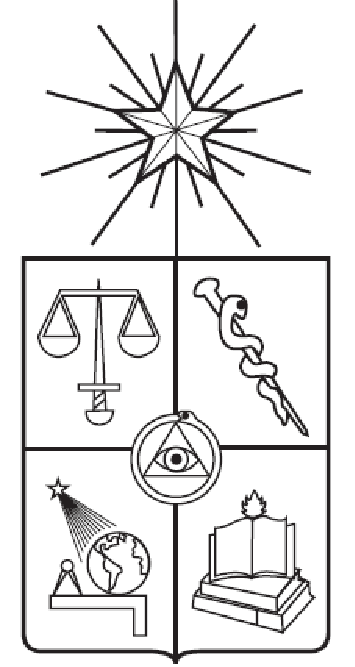
\includegraphics[width=1.5cm]{departamentos/uchile3} 
	\hspace{-0.2cm}
	\begin{tabular}{l}
		\small \scshape{\MakeUppercase{\nombreuniversidad}} \\
		\small \scshape{\MakeUppercase{\nombrefacultad}} \\
		\small \scshape{\MakeUppercase{\departamentouniversidad}} \\
		\vspace*{1cm}\mbox{}
	\end{tabular}
	
	\vfill
	\begin{center}
		\fontsize{8mm}{9mm}\selectfont
		\textcolor{\portraittitlecolor}{
			\noindent \titulodelinforme \\
			\noindent \temaatratar \\
		}
		\vspace*{1cm}
		\footnotesize{\codigodelcurso\ - \nombredelcurso} \\
		\vspace*{1.4cm}
	\end{center}
	
	\vfill
	\begin{center}
		\noindent \normalsize{\tablaintegrantes}
	\end{center}
}{
\ifthenelse{\equal{\portraitstyle}{style6}}{
	\setpagemargincm{\pagemarginleft}{\pagemargintop}{\pagemarginright}{\pagemarginbottom}
	\thispagestyle{empty}
	\begin{wrapfigure}{l}{0.3\textwidth}
		\vspace{-0.69cm}
		\noindent \hspace{-1.10cm} 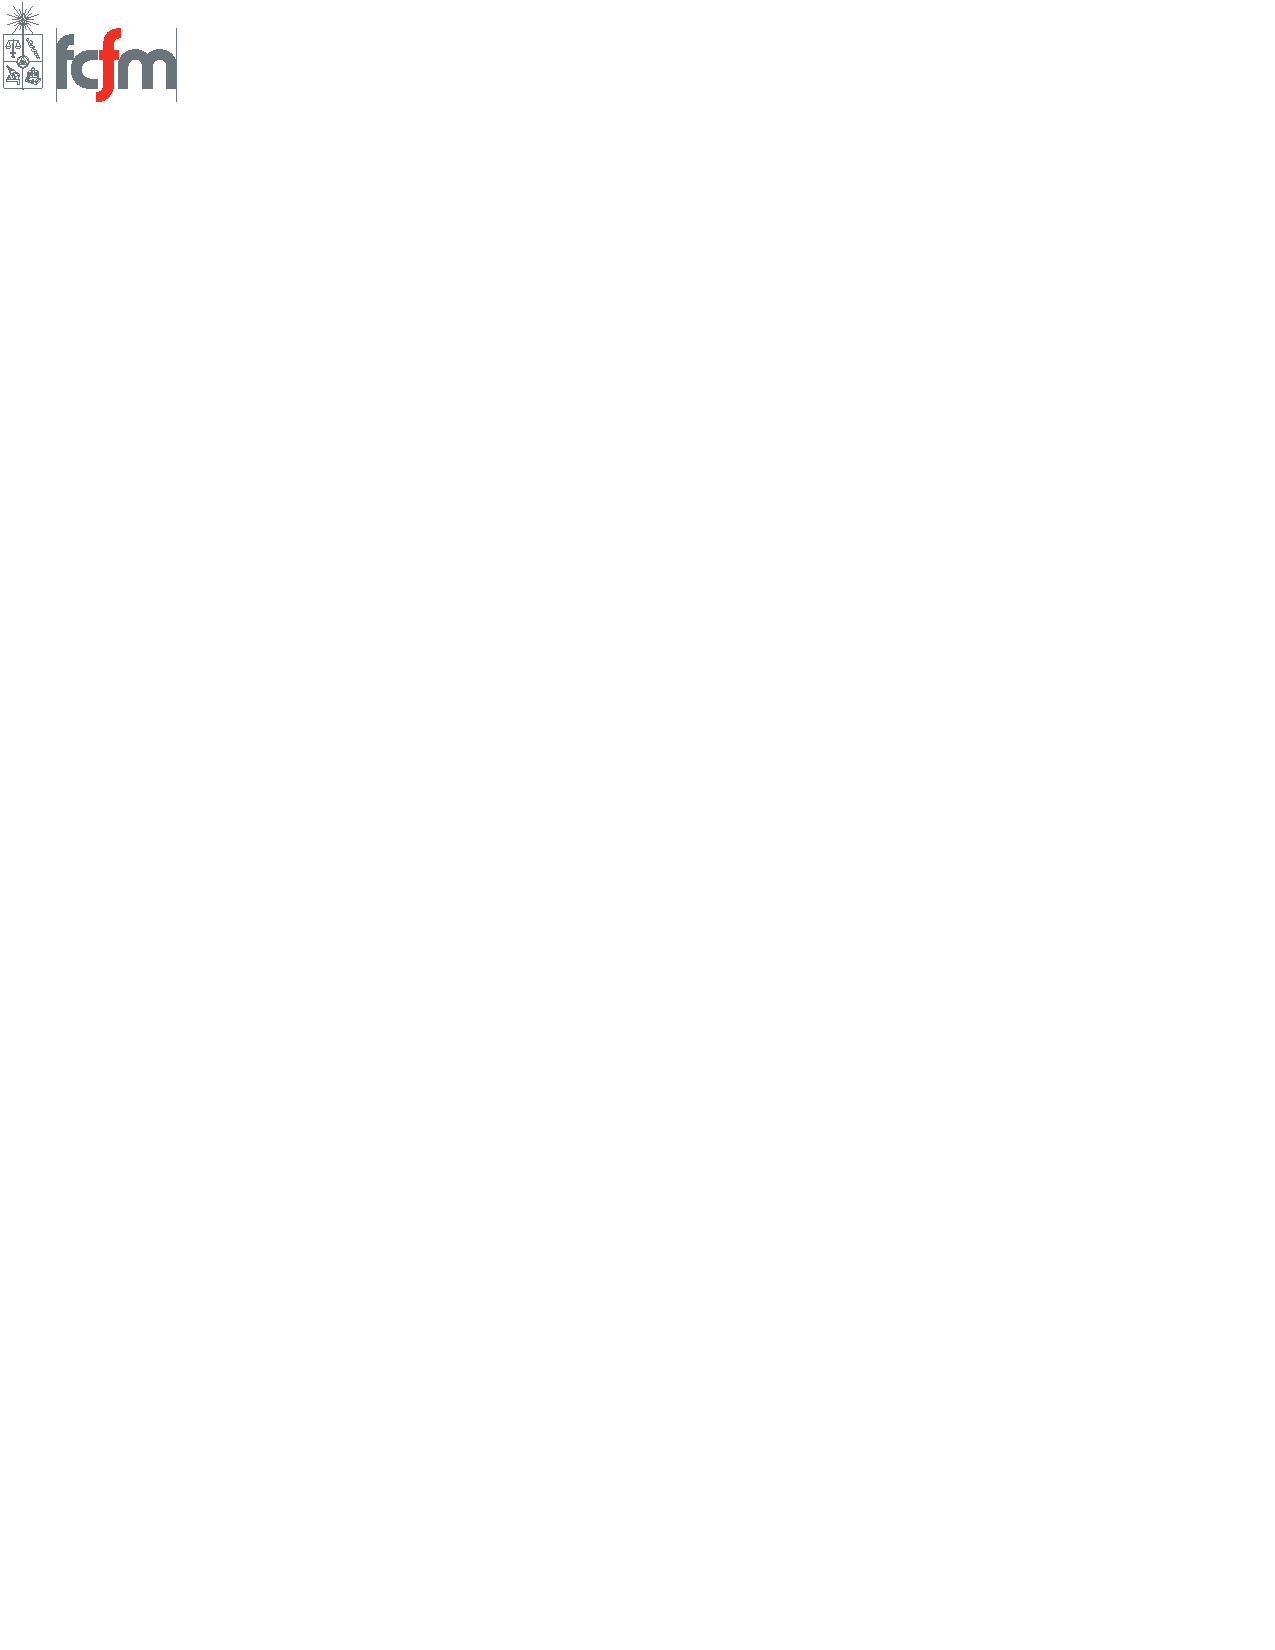
\includegraphics[scale=1.35]{departamentos/fcfm2}
	\end{wrapfigure}
	\hspace*{0.3cm}
	\noindent \textsc{\color{red} \hspace{-2.2cm} \departamentouniversidad} \\
	\hspace*{0.3cm}
	\noindent \textsc{\color{dgray} \hspace{-1.6cm} \nombrefacultad} \\
	\hspace*{0.3cm}
	\noindent \textsc{\color{dgray} \hspace{-1.6cm} \nombreuniversidad} \\
	\hspace*{0.3cm}
	\noindent \textsc{\color{dgray} \hspace{-1.6cm} \codigodelcurso \nombredelcurso}\\
	
	\vfill
	\begin{center}
		\vspace*{0.5cm}
		{\color{dgray} \Large \textbf{\MakeUppercase{\temaatratar}}} \\
		\noindent \rule{\linewidth}{0.3mm} ~ \\
		\Huge \textup \bfseries \textsc{\textcolor{\portraittitlecolor}{\titulodelinforme}} \\
		\noindent \rule{\linewidth}{0.3mm} ~ \\
	\end{center}
	\begin{minipage}{.5\textwidth}
		~
	\end{minipage}
	
	\vfill
	\begin{minipage}{1.0\textwidth}
		\begin{flushright}
			\noindent \tablaintegrantes
		\end{flushright}
	\end{minipage}
}{
\ifthenelse{\equal{\portraitstyle}{style7}}{
	\setpagemargincm{\pagemarginleft}{\pagemargintop}{\pagemarginright}{\pagemarginbottom}
	\thispagestyle{empty}
	\begin{center}
		\vspace*{-1.5cm}
		\includegraphics[scale=\imagendepartamentoescala]{\imagendepartamento}
		\hspace*{-0.15cm}
		\begin{tabular}{l}
			\vspace*{0.26cm}\mbox{} \\
			\small \scshape{\MakeUppercase{\nombreuniversidad}} \\
			\small \scshape{\MakeUppercase{\nombrefacultad}} \\
			\small \scshape{\MakeUppercase{\departamentouniversidad}} \\
			\vspace*{1.25cm}\mbox{}
		\end{tabular}
	\end{center}
	
	\vfill
	\begin{center}
		\noindent \rule{\textwidth}{0.4mm} \\ \vspace{0.3cm}
		{\huge \textcolor{\portraittitlecolor}{\titulodelinforme} \vspace{0.2cm} \\}
		\noindent \rule{\textwidth}{0.4mm} \\ \vspace{0.40cm}
		{\large \textcolor{\portraittitlecolor}{\temaatratar} \\}
	\end{center}
	
	\vfill
	\noindent
	\begin{minipage}{1.0\textwidth}
		\begin{flushright}
			\scshape{\tablaintegrantes}
		\end{flushright}
	\end{minipage}
}{
\ifthenelse{\equal{\portraitstyle}{style8}}{
	\setpagemargincm{\pagemarginleft}{\pagemargintop}{\pagemarginright}{\pagemarginbottom}
	\thispagestyle{empty}
	\begin{center}
		\vspace*{-1.0cm}
		\begin{tabular}{c}
			\includegraphics[scale=\imagendepartamentoescala]{\imagendepartamento} \vspace{0.5cm} \\
			\small \scshape{\MakeUppercase{\nombreuniversidad}} \\
			\small \scshape{\MakeUppercase{\nombrefacultad}} \\
			\small \scshape{\MakeUppercase{\departamentouniversidad}}
		\end{tabular}
	\end{center}
	
	\vfill
	\begin{center}
		\noindent \rule{\textwidth}{0.4mm} \\ \vspace{0.3cm}
		{\huge \textcolor{\portraittitlecolor}{\titulodelinforme} \vspace{0.2cm} \\}
		\noindent \rule{\textwidth}{0.4mm} \\ \vspace{0.40cm}
		{\large \textcolor{\portraittitlecolor}{\temaatratar} \\}
	\end{center}
	
	\vfill
	\noindent
	\begin{minipage}{1.0\textwidth}
		\begin{flushright}
			\scshape{\tablaintegrantes}
		\end{flushright}
	\end{minipage}
}{
\ifthenelse{\equal{\portraitstyle}{style9}}{
	\setpagemargincm{\pagemarginleft}{\pagemargintop}{\pagemarginright}{\pagemarginbottom}
	\thispagestyle{empty}
	\noindent \includegraphics[scale=\imagendepartamentoescala]{\imagendepartamento}
	\vfill
	\begin{center}
		\noindent \rule{\textwidth}{0.4mm} \\ \vspace{0.3cm}
		{\huge \textcolor{\portraittitlecolor}{\titulodelinforme} \vspace{0.2cm} \\}
		\noindent \rule{\textwidth}{0.4mm} \\ \vspace{0.35cm}
		{\large \textcolor{\portraittitlecolor}{\temaatratar} \\}
	\end{center}
	
	\vfill
	\begin{center}
		\begin{tabular}{c}
			\small \scshape{\MakeUppercase{\nombreuniversidad}} \\
			\small \scshape{\MakeUppercase{\nombrefacultad}} \\
			\small \scshape{\MakeUppercase{\departamentouniversidad}}
		\end{tabular}
	\end{center}
	
	\vfill
	\begin{center}
		\indent \scshape{\tablaintegrantes}
	\end{center}
}{
\ifthenelse{\equal{\portraitstyle}{style10}}{
	\setpagemargincm{\pagemarginleft}{\pagemargintop}{\pagemarginright}{\pagemarginbottom}
	\thispagestyle{empty}
	
	~ \\
	\vfill
	\begin{center}
		\noindent {\large \textsc{\nombreuniversidad, \departamentouniversidad}}
		\vspace{1.0cm}
	\end{center}
	
	\vfill
	\begin{center}
		\noindent {\large \scshape{\nombredelcurso}} \vspace{0.5cm} \\
		\noindent {\large \scshape{\codigodelcurso}} \vspace{0.5cm} \\
		\noindent \rule{\textwidth}{0.4mm} \\ \vspace{0.3cm}
		{\huge \bfseries \textcolor{\portraittitlecolor}{\titulodelinforme} \vspace{0.2cm} \\}
		\noindent \rule{\textwidth}{0.4mm} \\ \vspace{2.5cm}
	\end{center}
	
	\vfill
	\begin{center}
		\indent \tablaintegrantes
	\end{center}
	
	\vfill
	~ \\
}{
\ifthenelse{\equal{\portraitstyle}{style11}}{
	\setpagemargincm{\pagemarginleft}{\pagemargintop}{\pagemarginright}{\pagemarginbottom}
	\thispagestyle{empty}
	\begin{center}
		\vspace*{-1.0cm}
		\scshape{\nombreuniversidad} \\
		\scshape{\nombrefacultad} \\
		\scshape{\departamentouniversidad}
	\end{center}
	
	\vfill
	\begin{center}
		{\setstretch{1.2} \fontsize{21pt}{22pt} \selectfont \textcolor{\portraittitlecolor}{\scshape{\titulodelinforme}} \vspace{0.5cm}} \\
		{\fontsize{13pt}{10pt} \selectfont \textcolor{\portraittitlecolor}{\scshape{\temaatratar}}}
	\end{center}
	
	\vfill
	\begin{center}
		\indent \tablaintegrantes
	\end{center}
}{
\ifthenelse{\equal{\portraitstyle}{style12}}{
	\setpagemargincm{\pagemarginleft}{\pagemargintop}{\pagemarginright}{\pagemarginbottom}
	\thispagestyle{empty}
	\begin{center}
		\vspace*{-1.0cm}
		\includegraphics[scale=\imagendepartamentoescala]{\imagendepartamento}
	\end{center}

	\vfill
	\begin{center}
		{\bf \Huge \scshape{\textcolor{\portraittitlecolor}{\titulodelinforme}} \vspace{0.3cm}} \\
		{\bf \Large \textcolor{\portraittitlecolor}{\temaatratar}}
	\end{center}
	
	\vfill
	\begin{flushright}
		\noindent \tablaintegrantes
	\end{flushright}

	\vspace{0.5cm}
	\noindent \rule{\textwidth}{0.4mm}
	\begin{center}
		\scshape{\nombreuniversidad, \nombrefacultad} \\
		\scshape{\departamentouniversidad}
	\end{center}
}{
\ifthenelse{\equal{\portraitstyle}{style13}}{
	\setpagemargincm{\pagemarginleft}{\pagemargintop}{\pagemarginright}{\pagemarginbottom}
	\thispagestyle{empty}
	\noindent
	\vspace*{-1.5cm}
	\begin{flushleft}
		\begin{minipage}{0.65\textwidth}
			{\fontsize{3.5mm}{0.5mm} \selectfont \noindent  \textsf{\nombreuniversidad, \nombrefacultad}} \\
			\noindent {\fontsize{3.0mm}{0.5mm} \selectfont \textsf{\departamentouniversidad} \vspace{-0.2cm}} \\
			\noindent \textcolor{lgray}{\rule{\textwidth}{0.3mm}}
		\end{minipage}
	\end{flushleft}
	\vspace*{-2.15cm}
	\begin{flushright}
		\begin{minipage}{0.3\textwidth}
			\noindent \includegraphics[width=1.0\textwidth]{\imagendepartamento}
		\end{minipage}
	\end{flushright}
	
	\vfill
	\begin{center}
		\begin{minipage}{0.9\textwidth}
			\begin{framed}
				\LARGE
				\vspace{1cm}
				\centering \textcolor{\portraittitlecolor}{\textbf{\titulodelinforme}}
				\vspace{1cm}
			\end{framed}
		\end{minipage}
	\end{center}
	
	\vfill
	\begin{flushright}
		\noindent \textsf{\tablaintegrantes}
	\end{flushright}
}{
\ifthenelse{\equal{\portraitstyle}{style14}}{
	\setpagemargincm{\pagemarginleft}{\pagemargintop}{\pagemarginright}{\pagemarginbottom}
	\thispagestyle{empty}
	\noindent
	\begin{flushleft}
		\vspace*{-1.0cm}
		\noindent \includegraphics[scale=\imagendepartamentoescala]{\imagendepartamento} \\
	\end{flushleft}
	
	\vfill
	{\bf \huge \noindent \textcolor{\portraittitlecolor}{\textsf{\MakeUppercase{\titulodelinforme}} \vspace*{0.05cm}}} \\
	{\bf \large \noindent \textcolor{\portraittitlecolor}{\textsf{\MakeUppercase{\temaatratar}}}} \\
	
	\vfill
	\begin{flushright}
		\noindent \textsf{\tablaintegrantes}
	\end{flushright}
}{
\ifthenelse{\equal{\portraitstyle}{style15}}{
	\setpagemargincm{\pagemarginleft}{\pagemargintop}{\pagemarginright}{\pagemarginbottom}
	\thispagestyle{empty}
	
	% Se chequean variables propias de la portada
	\checkextravarexist{\imagenextraportada}{}
	\checkextravarexist{\imagenextraportadaescala}{}
	
	\vspace*{-1.5cm}
	\noindent \begin{minipage}{0.8\textwidth}
		\noindent \begin{minipage}{0.22\textwidth}
			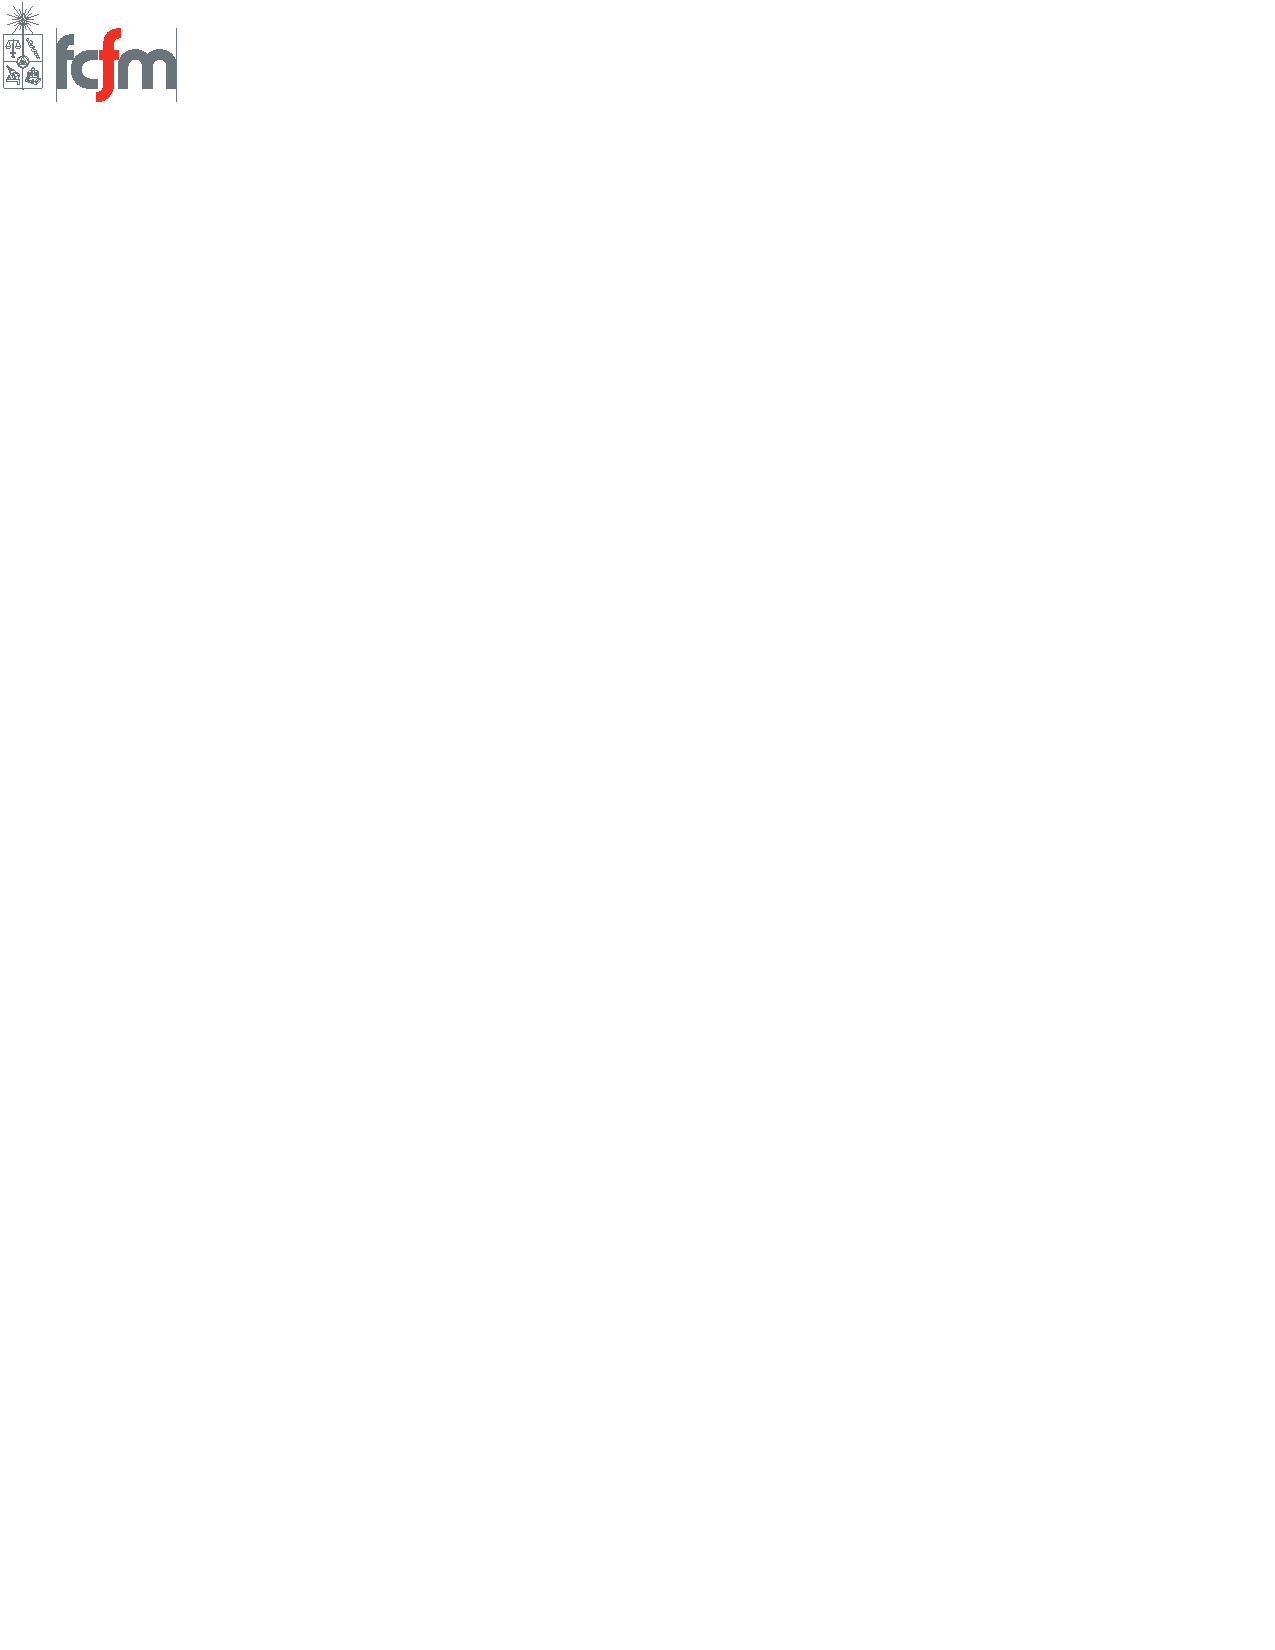
\includegraphics[scale=1.0]{departamentos/fcfm2} \\
		\end{minipage}
		\begin{minipage}{0.6\textwidth}
			\begin{flushleft}
				\textsc{
				\begin{tabular}{l}
					{\small \nombreuniversidad} \\
					{\small \nombrefacultad} \\
					{\small \departamentouniversidad}
				\end{tabular}
				}
			\end{flushleft}
		\end{minipage}
	\end{minipage}
	\noindent \begin{minipage}{0.2\textwidth}
		\begin{flushright}
			\ifthenelse{\isundefined{\imagenextraportada}}{}{
				\ifthenelse{\isundefined{\imagenextraportadaescala}}{}{
					\noindent \includegraphics[scale=\imagenextraportadaescala]{\imagenextraportada} \\
				}
			}
		\end{flushright}
	\end{minipage}
	
	\vfill
	\begin{center}
		{\fontsize{25pt}{15pt} \selectfont \textcolor{\portraittitlecolor}{\textbf{\titulodelinforme}} \vspace{0.7cm}} \\
		{\Large \textcolor{\portraittitlecolor}{\temaatratar}}
	\end{center}
	
	\vfill
	\begin{center}
		\noindent \tablaintegrantes
	\end{center}
}{
\ifthenelse{\equal{\portraitstyle}{style16}}{
	\setpagemargincm{\pagemarginleft}{\pagemargintop}{\pagemarginright}{\pagemarginbottom}
	
	\checkextravarexist{\imagenfondoportada}{Defina el fondo de la portada en el bloque INFORMACION DEL DOCUMENTO. Por defecto se uso la portada ubicada en ejemplos}
	\ifthenelse{\isundefined{\imagenfondoportada}}{
		\def\imagenfondoportada {ejemplos/background-1}
	}{}
	\checkextravarexist{\colorbloqueportada}{Defina el color del bloque del titulo de la portada en el bloque INFORMACION DEL DOCUMENTO. Por defecto se uso el color ocre}
	\ifthenelse{\isundefined{\imagenfondoportada}}{
		\def\imagenfondoportada {ejemplos/background-1}
	}{}
	\ifthenelse{\isundefined{\colorbloqueportada}}{
		\def\colorbloqueportada {ocre}
	}{}
	
	\begingroup
	\thispagestyle{empty}
	\begin{tikzpicture}[remember picture,overlay]
		\node[inner sep=0pt] (background) at (current page.center) {\includegraphics[width=\paperwidth]{\imagenfondoportada}};
		\draw (current page.center) node [fill=\colorbloqueportada!30!white,fill opacity=0.6,text opacity=1,inner sep=1cm]{\Huge\centering\bfseries\sffamily\parbox[c][][t]{\paperwidth}{
				\centering \textcolor{\portraittitlecolor}{\titulodelinforme} \\ [10pt]
				{\Large \temaatratar} \\ [25pt]
				{\huge \autordeldocumento}}};
	\end{tikzpicture}
	\vfill
	\endgroup
}{
\ifthenelse{\equal{\portraitstyle}{\bgtemplatetestcode}}{
	\setpagemargincm{\pagemarginleft}{\pagemargintop}{\pagemarginright}{\pagemarginbottom}
	\pagestyle{empty}
	\pagecolor{lbrown}
	\begin{center}
		\vspace*{-1.0cm}
		\scshape{\nombreuniversidad} \\
		\scshape{\nombrefacultad} \\
		\scshape{\departamentouniversidad}
	\end{center}
	
	~ \\
	\begin{center}
		\bgtemplatetestimg
	\end{center}

	\begin{center}
		\vspace*{-6cm}
		{\setstretch{1.2} \fontsize{25pt}{22pt} \selectfont \textcolor{\portraittitlecolor}{\scshape{\titulodelinforme}} \vspace{0.5cm}} \\
		{\fontsize{15pt}{10pt} \selectfont \textcolor{\portraittitlecolor}{\scshape{\temaatratar}}}
	\end{center}

	\vfill
	\begin{flushright}
		\noindent \tablaintegrantes
	\end{flushright}
	\newpage
	\pagecolor{white}
}{
	\throwbadconfigondoc{Estilo de portada incorrecto}{\portraitstyle}{style1 .. style16}}}}}}}}}}}}}}}}}
}

% Añade una página en blanco al imprimir por las dos caras
\ifthenelse{\equal{\addemptypagetwosides}{true}}{
	\newpage
	\null
	\thispagestyle{empty}
	\renewcommand{\thepage}{}
	\newpage}{
}


% CONFIGURACIÓN DE PÁGINA Y ENCABEZADOS
% Template:     Informe/Reporte LaTeX
% Documento:    Configuración de página
% Versión:      4.7.3 (05/02/2018)
% Codificación: UTF-8
%
% Autor: Pablo Pizarro R.
%        Facultad de Ciencias Físicas y Matemáticas
%        Universidad de Chile
%        pablo.pizarro@ing.uchile.cl, ppizarror.com
%
% Manual template: [http://latex.ppizarror.com/Template-Informe/]
% Licencia MIT:    [https://opensource.org/licenses/MIT/]

% Numeración de páginas
\newpage
\ifthenelse{\equal{\romanpageuppercase}{true}}{
	\pagenumbering{Roman}
}{
	\pagenumbering{roman}
}
\setcounter{page}{1}
\setcounter{footnote}{1}

% Márgenes de páginas y tablas
\setpagemargincm{\pagemarginleft}{\pagemargintop}{\pagemarginright}{\pagemarginbottom}
\def\arraystretch{\tablepadding} % Se ajusta el padding de las tablas

% Se define el punto decimal
\ifthenelse{\equal{\pointdecimal}{true}}{
	\decimalpoint}{
}

% Definición de nombres de objetos
\renewcommand{\appendixname}{\nomltappendixsection} % Nombre del anexo (título)
\renewcommand{\appendixpagename}{\nameappendixsection} % Nombre del anexo en índice
\renewcommand{\appendixtocname}{\nameappendixsection} % Nombre del anexo en índice
\renewcommand{\contentsname}{\nomltcont}  % Nombre del índice
\renewcommand{\figurename}{\nomltwfigure} % Nombre de la leyenda de las fig.
\renewcommand{\listfigurename}{\nomltfigure} % Nombre del índice de figuras
\renewcommand{\listtablename}{\nomlttable} % Nombre del índice de tablas
\renewcommand{\lstlistingname}{\nomltwsrc} % Nombre leyenda del código fuente
\renewcommand{\lstlistlistingname}{\nomltsrc} % Nombre índice código fuente
\renewcommand{\refname}{\namereferences} % Nombre de las referencias
\renewcommand{\tablename}{\nomltwtable} % Nombre de la leyenda de tablas

% Estilo de títulos
\sectionfont{\color{\titlecolor} \fontsizetitle \styletitle \selectfont}
\subsectionfont{\color{\subtitlecolor} \fontsizesubtitle \stylesubtitle \selectfont}
\subsubsectionfont{\color{\subsubtitlecolor} \fontsizesubsubtitle \stylesubsubtitle \selectfont}

% Se crean los header-footer
\ifthenelse{\equal{\hfstyle}{style1}}{
	\pagestyle{fancy} \fancyhf{}
	\fancyhead[L]{\nouppercase{\rightmark}}
	\fancyhead[R]{\small \rm \thepage}
	\fancyfoot[L]{\small \rm \textit{\titulodelinforme}}
	\fancyfoot[R]{\small \rm \textit{\codigodelcurso \nombredelcurso}}
	\renewcommand{\headrulewidth}{0.5pt}
	\renewcommand{\footrulewidth}{0.5pt}
	\renewcommand{\sectionmark}[1]{\markboth{#1}{}}
}{
\ifthenelse{\equal{\hfstyle}{style2}}{
	\pagestyle{fancy} \fancyhf{}
	\fancyhead[L]{\nouppercase{\rightmark}}
	\fancyhead[R]{\small \rm \thepage}
	\fancyfoot[L]{\small \rm \textit{\titulodelinforme}}
	\fancyfoot[R]{\small \rm \textit{\codigodelcurso \nombredelcurso}}
	\renewcommand{\headrulewidth}{0.5pt}
	\renewcommand{\footrulewidth}{0pt}
	\renewcommand{\sectionmark}[1]{\markboth{#1}{}}
}{
\ifthenelse{\equal{\hfstyle}{style3}}{
	\pagestyle{fancy} \fancyhf{}
	\fancyhead[L]{
		\small \rm \textit{\codigodelcurso \nombredelcurso}
		\vspace{0.04cm}
	}
	\fancyhead[R]{
		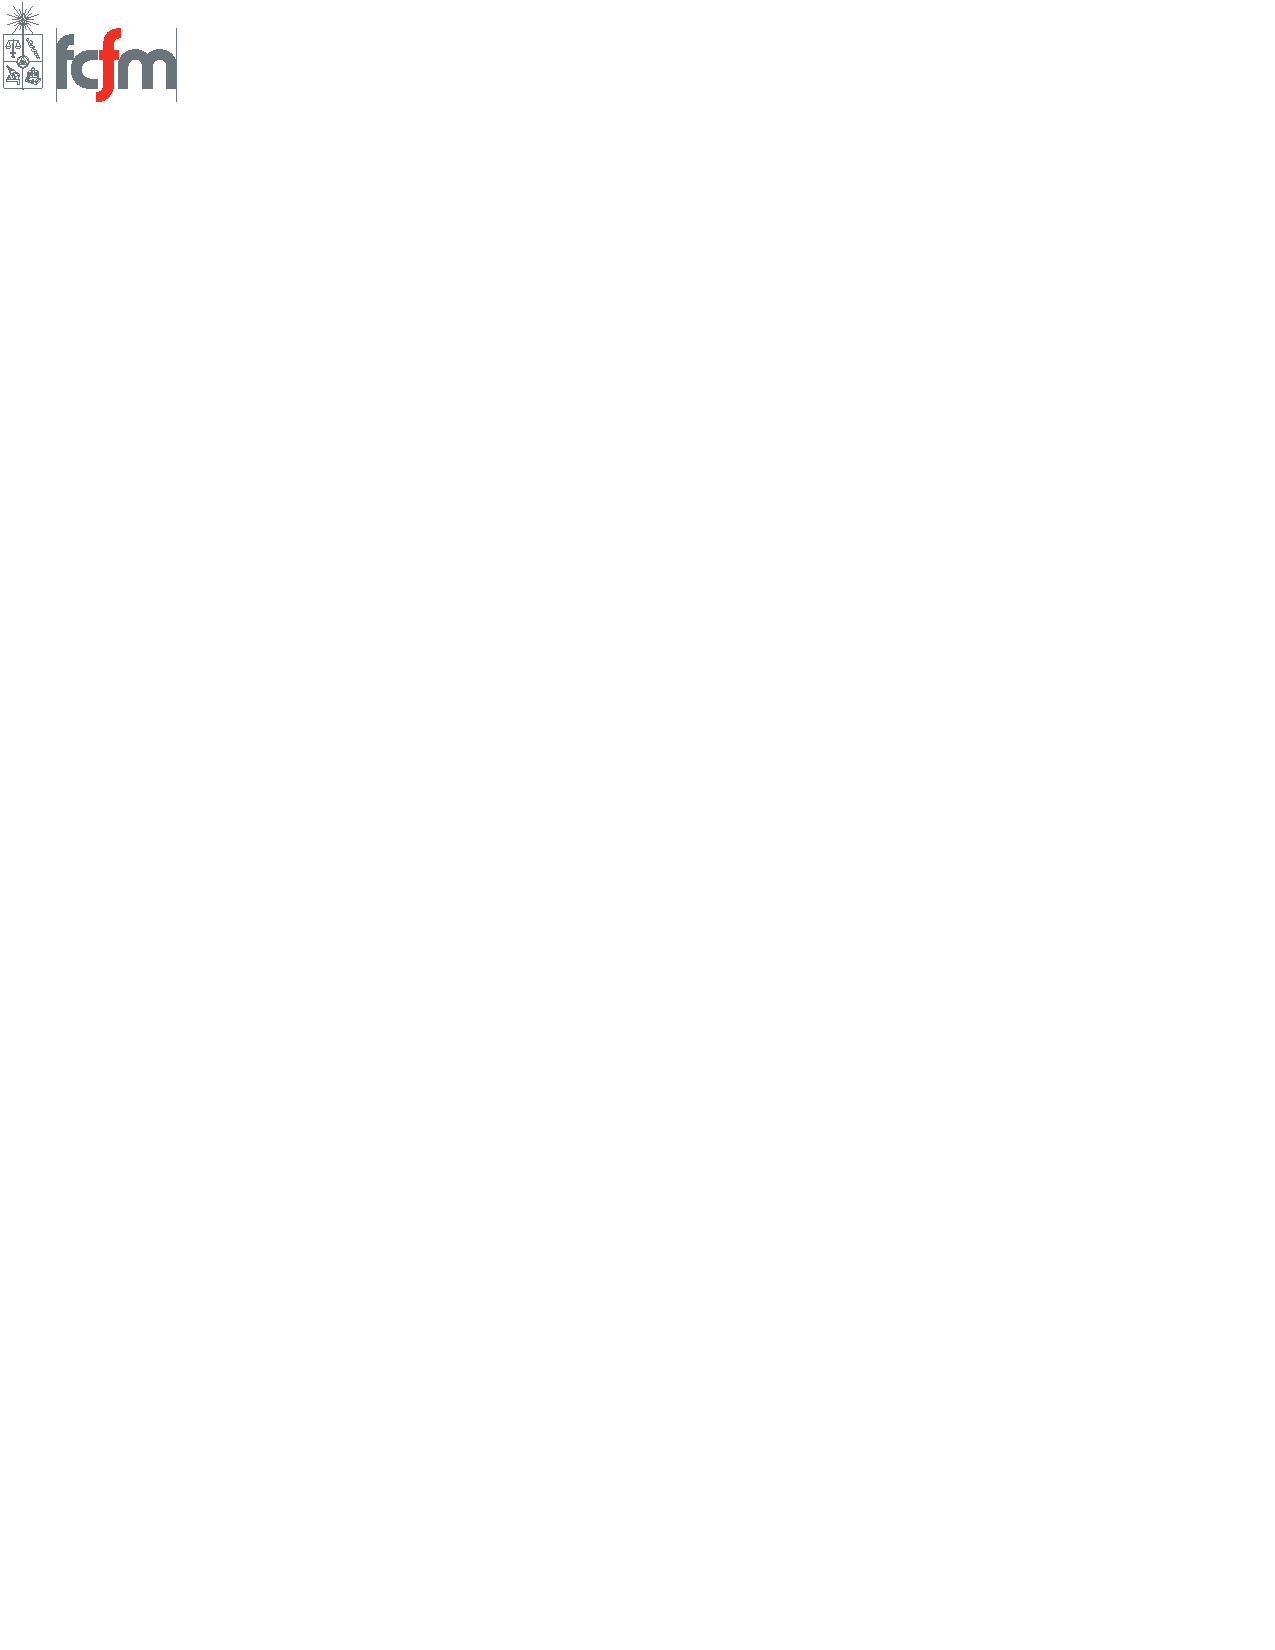
\includegraphics[width=1.2cm]{departamentos/fcfm2}
		\vspace{-0.10cm}
	}
	\fancyfoot[C]{\thepage}
	\renewcommand{\headrulewidth}{0.5pt}
	\renewcommand{\footrulewidth}{0pt}
}{
\ifthenelse{\equal{\hfstyle}{style4}}{
	\pagestyle{fancy} \fancyhf{}
	\fancyhead[L]{\nouppercase{\rightmark}}
	\fancyhead[R]{}
	\fancyfoot[C]{\small \rm \thepage}
	\renewcommand{\headrulewidth}{0.5pt}
	\renewcommand{\footrulewidth}{0pt}
	\renewcommand{\sectionmark}[1]{\markboth{#1}{}}
}{
\ifthenelse{\equal{\hfstyle}{style5}}{
	\pagestyle{fancy} \fancyhf{}
	\fancyhead[L]{\codigodelcurso \nombredelcurso}
	\fancyhead[R]{\nouppercase{\rightmark}}
	\fancyfoot[L]{\departamentouniversidad, \nombreuniversidad}
	\fancyfoot[R]{\small \rm \thepage}
	\renewcommand{\headrulewidth}{0pt}
	\renewcommand{\footrulewidth}{0pt}
	\renewcommand{\sectionmark}[1]{\markboth{#1}{}}
}{
\ifthenelse{\equal{\hfstyle}{style6}}{
	\pagestyle{fancy} \fancyhf{}
	\fancyfoot[L]{\departamentouniversidad}
	\fancyfoot[C]{\thepage}
	\fancyfoot[R]{\nombreuniversidad}
	\renewcommand{\headrulewidth}{0pt}
	\renewcommand{\footrulewidth}{0pt}
	\setlength{\headheight}{49pt}
}{
\ifthenelse{\equal{\hfstyle}{style7}}{
	\pagestyle{fancy} \fancyhf{}
	\fancyfoot[C]{\thepage}
	\renewcommand{\headrulewidth}{0pt}
	\renewcommand{\footrulewidth}{0pt}
	\setlength{\headheight}{49pt}
}{
\ifthenelse{\equal{\hfstyle}{style8}}{
	\pagestyle{fancy} \fancyhf{}
	\fancyfoot[R]{\thepage}
	\renewcommand{\headrulewidth}{0pt}
	\renewcommand{\footrulewidth}{0pt}
	\setlength{\headheight}{49pt}
}{
	\throwbadconfigondoc{Estilo de header-footer incorrecto}{\hfstyle}{style1 .. style8}}}}}}}}
}

% Muestra los números de línea
\ifthenelse{\equal{\showlinenumbers}{true}}{
	\linenumbers}{
}


\begin{resumen}
  En este paper, se detalla una implementación del algoritmo de Felzenszwalb de segmentación de imágenes basada en grafos. Luego se discuten los resultados y se proponen posibles mejoras a la implementación realizada.
\end{resumen}

% CONFIGURACIONES FINALES
% Template:     Informe/Reporte LaTeX
% Documento:    Configuraciones finales
% Versión:      4.7.3 (05/02/2018)
% Codificación: UTF-8
%
% Autor: Pablo Pizarro R.
%        Facultad de Ciencias Físicas y Matemáticas
%        Universidad de Chile
%        pablo.pizarro@ing.uchile.cl, ppizarror.com
%
% Manual template: [http://latex.ppizarror.com/Template-Informe/]
% Licencia MIT:    [https://opensource.org/licenses/MIT/]

% Se reestablecen headers y footers
\markboth{}{}
\newpage
\ifthenelse{\equal{\hfstyle}{style1}}{
	\fancyhead[L]{\nouppercase{\leftmark}}}{
}
\ifthenelse{\equal{\hfstyle}{style2}}{
	\fancyhead[L]{\nouppercase{\leftmark}}}{
}
\ifthenelse{\equal{\hfstyle}{style4}}{
	\fancyhead[L]{\nouppercase{\leftmark}}}{
}
\ifthenelse{\equal{\hfstyle}{style5}}{
	\fancyhead[R]{\nouppercase{\leftmark}}}{
}

% Estilo de títulos
\sectionfont{\color{\titlecolor} \fontsizetitle \styletitle \selectfont}
\subsectionfont{\color{\subtitlecolor} \fontsizesubtitle \stylesubtitle \selectfont}
\subsubsectionfont{\color{\subsubtitlecolor} \fontsizesubsubtitle \stylesubsubtitle \selectfont}

% Numeración de objetos
\ifthenelse{\equal{\showsectioncaption}{none}}{
}{
\ifthenelse{\equal{\showsectioncaption}{sec}}{
	\counterwithin{equation}{section}   % Añade número de sección a las ecuaciones
	\counterwithin{figure}{section}     % Añade número de sección a las figuras
	\counterwithin{lstlisting}{section} % Añade número de sección a los códigos
	\counterwithin{table}{section}      % Añade número de sección a las tablas
}{
\ifthenelse{\equal{\showsectioncaption}{ssec}}{
	\counterwithin{equation}{subsection}   % Añade número de subsección a las ecuaciones
	\counterwithin{figure}{subsection}     % Añade número de subsección a las figuras
	\counterwithin{lstlisting}{subsection} % Añade número de subsección a los códigos
	\counterwithin{table}{subsection}      % Añade número de subsección a las tablas
}{
\ifthenelse{\equal{\showsectioncaption}{sssec}}{
	\counterwithin{equation}{subsubsection}   % Añade número de subsección a las ecuaciones
	\counterwithin{figure}{subsubsection}     % Añade número de subsección a las figuras
	\counterwithin{lstlisting}{subsubsection} % Añade número de subsección a los códigos
	\counterwithin{table}{subsubsection}      % Añade número de subsección a las tablas
}{
\throwbadconfig{Valor configuracion incorrecto}{\showsectioncaption}{none,sec,ssec,sssec}
}}}}

% Se reestablecen números de página y secciones
\renewcommand{\thepage}{\arabic{page}}
\setcounter{page}{1}
\setcounter{section}{0}
\setcounter{footnote}{0}

% Muestra los números de línea
\ifthenelse{\equal{\showlinenumbers}{true}}{
	\linenumbers}{
}


% ======================= INICIO DEL DOCUMENTO =======================

\section{Introducción}
  El algoritmo de Felzenszwalb se basa en interpretar una imagen como un grafo no direccionado con pesos. Cada pixel de la imagen se traduce en un vértice del grafo, y existen aristas entre todos los pixeles vecinos (puede ser en el sentido 4-conectado o 8-conectado, en este paper se utilizó el caso 8-conectado.). Luego se utilizan métricas de diferencia interna dentro de un cluster de vértices y de diferencia interna mínima entre clusters para tener una condición de mezcla de clusters. Iterando sobre las aristas del grafo se evalúa esta condición y se genera una segmentación de la imagen dada.
  
\section{Desarrollo}
  La implementación de este algoritmo se realizó mediante 3 clases, una que contiene información sobre la imagen y que realiza en algoritmo en sí, y una clase para representar un vértice, soportando operaciones de la estructura de datos Union-Find, y una otra para representar una arista en el grafo.

  La clase que representa un vértice, \texttt{Vertex}, define los siguientes campos y métodos:
  \begin{itemize}
    \item Campos:
    \begin{itemize}
      \item \texttt{coordinates}: Coordenadas del vértice en la imágen. Usado para verificar la igualdad entre dos vértices.
      \item \texttt{parent}: Define el padre del nodo en la estructura Union-Find.
    \end{itemize}
    \item Métodos:
    \begin{itemize}
      \item \texttt{find}: Realiza la búsqueda de la raíz del cluster de la estructura Union-Find al que pertenece el nodo. Se realiza además compresión de camino, para que las próximas búsquedas desde ese nodo y sus ancestros tomen tiempo constante.
      \item \texttt{unite}: Recibe como parámetro otro nodo. Hace que el padre del nodo entregado sea el nodo que recibe el método. Se asume que el usuario entrega las raíces de dos distintos clusters para evitar generación de ciclos en la estructura.
    \end{itemize}
  \end{itemize}
  Estas operaciones de Union-Find necesitan que todos los vértices relevantes se mantengan en memoria al mismo tiempo, para no perder las conexiones en la estructura Union-Find.

  La clase principal tiene los siguientes campos:
  \begin{itemize}
    \item \texttt{image}: Campo que guarda la imagen sobre la cual se realizará la segmentación.
    \item \texttt{vertices}: Matriz del mismo ancho y alto que la imágen, donde cada coordenada almacena un objeto de la clase \texttt{Vertex}, para poder mantenerlos en memoria y que no sean borrados al perder sus referencias.
    \item \texttt{clusters}: Diccionario donde las llaves son 2-tuplas que corresponden a coordenadas de la imágen, y los valores son una lista de 2-tuplas que tienen como raíz en la estructura Union-Find, la llave que les apunta.
    \item \texttt{edges}: Diccionario donde las llaves son 2-tuplas que corresponden a un par de coordenadas de la imágen, y los valores son objetos Edge, los cuales simplemente almacenan el peso correspondiente a esa arista y los dos vértices que la forman.
  \end{itemize}

  La inicialización de la clase comienza llenando la matriz \texttt{vertices} con cada coordenada teniendo un objeto \texttt{Vertex} con la coordenada de aquella celda. El diccionario clusters comienza inicializado con todas las coordenadas de la imágen, y una lista conteniendo la misma coordenada, como pares llave-valor. Finalmente, el diccionario edges fue el más problemático, pues este ocupaba mucha memoria si se almacenaban todas las aristas de la imágen. Para resolver esto se decidió realizar durante el parsing de estos bordes la unión de vértices donde la arista que los conectaba tenía peso 0. Esto es válido según el algoritmo, pues la evaluación de condición para unir distintos clusters se realiza en el set de aristas, en orden no creciente, por lo que las aristas con peso 0 siempre irán primero (notar que ninguna arista puede tener peso negativo). Además de esto, cualquier arista de peso 0 siempre fuerza una unión, para cualquier valor de $k > 0$. De este modo, en la inicialización de la clase sólo se guardan los valores de las aristas no nulos, y se unen todos los nodos con aristas de peso 0.

  Otro punto importante es que para evitar la duplicación de elementos en el diccionario de aristas, para un par de vértices $v_i, v_j$, sólo se almacenaba en el diccionario la tupla $(v_i, v_j)$, y se implementó una función que buscaba si existía un par dado en el diccionario, buscando las dos posibles permutaciones como llave. Si no se encontraba se retornaba 0.

  Esta clase define además métodos para el cálculo de las métricas de cada cluster, incluyendo el cálculo del MST de un cluster y la diferencia interna mínima entre dos clusters.
  
\section{Resultados}
  La solucuón implementada logra calcular las aristas de la imágen relativamente rápido, pero al iterar sobre las aristas no-cero, suele frenarse bastante luego de cierto tiempo. Se sospecha que esto es debido a falta de memoria, por lo que la colección de basura frena la ejecución del programa.

  Además, la segmentación generada no es muy buena, de hecho, no se logran ver los objetos originales de la imágen, por lo que probablemente exista una falla en el cálculo de distancias en la imágen o en la obtención del MST de ésta, por lo que se evalúa mal la condición de mezcla de clusters.

  A continuación se presentan los resultados de la segmentación variando algunos parámetros y para las imágenes entregadas, y las buscadas.

  \subsection{Efecto de el parámetro $k$}
    Se probó la segmentación sobre la imágen 1 para $k\in(150, 500, 1000)$, obteniendo los siguientes resultados.

    \begin{figure}[H]
      \centering
      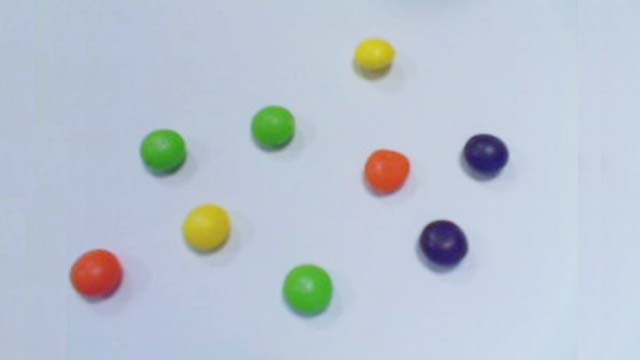
\includegraphics[width=0.3\textwidth]{images/image_1}
      \vspace{0.5cm}

      \begin{minipage}{0.3\textwidth}
        \centering
        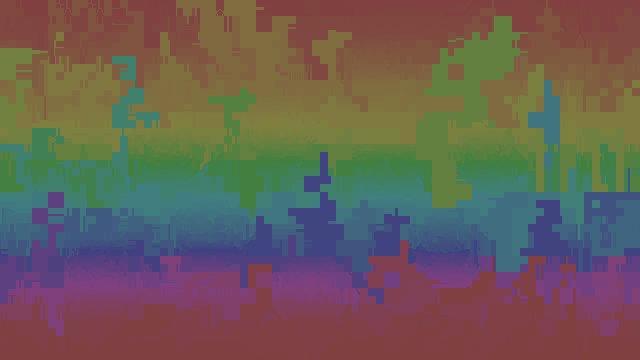
\includegraphics[width=0.8\textwidth]{images/result_a}
      \end{minipage}
      \begin{minipage}{0.3\textwidth}
        \centering
        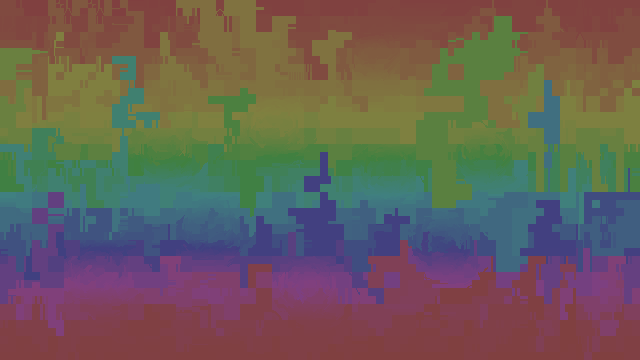
\includegraphics[width=0.8\textwidth]{images/result_b}
      \end{minipage}
      \begin{minipage}{0.3\textwidth}
        \centering
        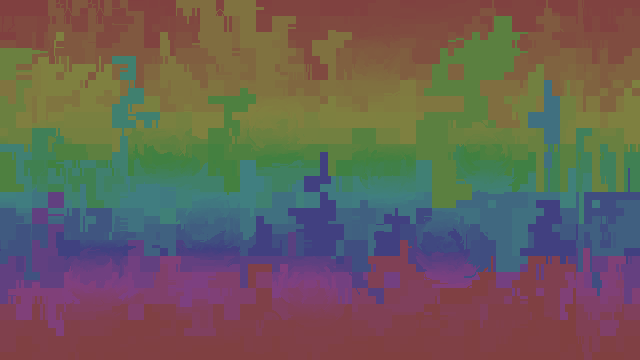
\includegraphics[width=0.8\textwidth]{images/result_c}
      \end{minipage}
      \caption{Resultados obtenidos para la imagen 1. De derecha a izquiera, $k=150$, $k=500$ y $k=1000$.}
    \end{figure}

    No se logra ver mucho cambio entre los distintos valores de $k$, esto probablemente se deba al mismo error que causa que las segmentaciones generadas no tengan mucho sentido. Cada una de las segmentaciones tomó alrededor de 1 hora en generarse.

  \subsection{Resultados para imágenes entregadas}
    Sólo se logró generar segmentaciones sólo para las imágenes 1, 2 y 3, debido a quela resolución de las imágenes 4 y 5 era demasiado grande, lo que hacía poco viable realizar este análisis sobre ellas, dado que tomarían sobre 6 horas cada una.

    \begin{figure}[H]
      \centering
      \begin{minipage}{0.4\textwidth}
        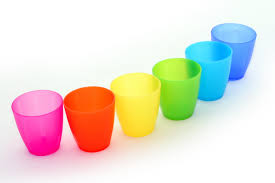
\includegraphics[width=0.8\textwidth]{images/image_2}
      \end{minipage}
      \begin{minipage}{0.4\textwidth}
        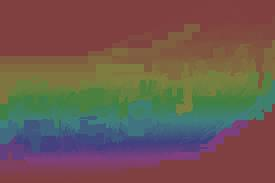
\includegraphics[width=0.8\textwidth]{images/result_image2}
      \end{minipage}
      \caption{A la izquierda la imágen 2, y la derecha el resultado de su segmentación. Esta tomó 8 minutos en generarse.}
    \end{figure}

    \begin{figure}[H]
      \centering
      \begin{minipage}{0.4\textwidth}
        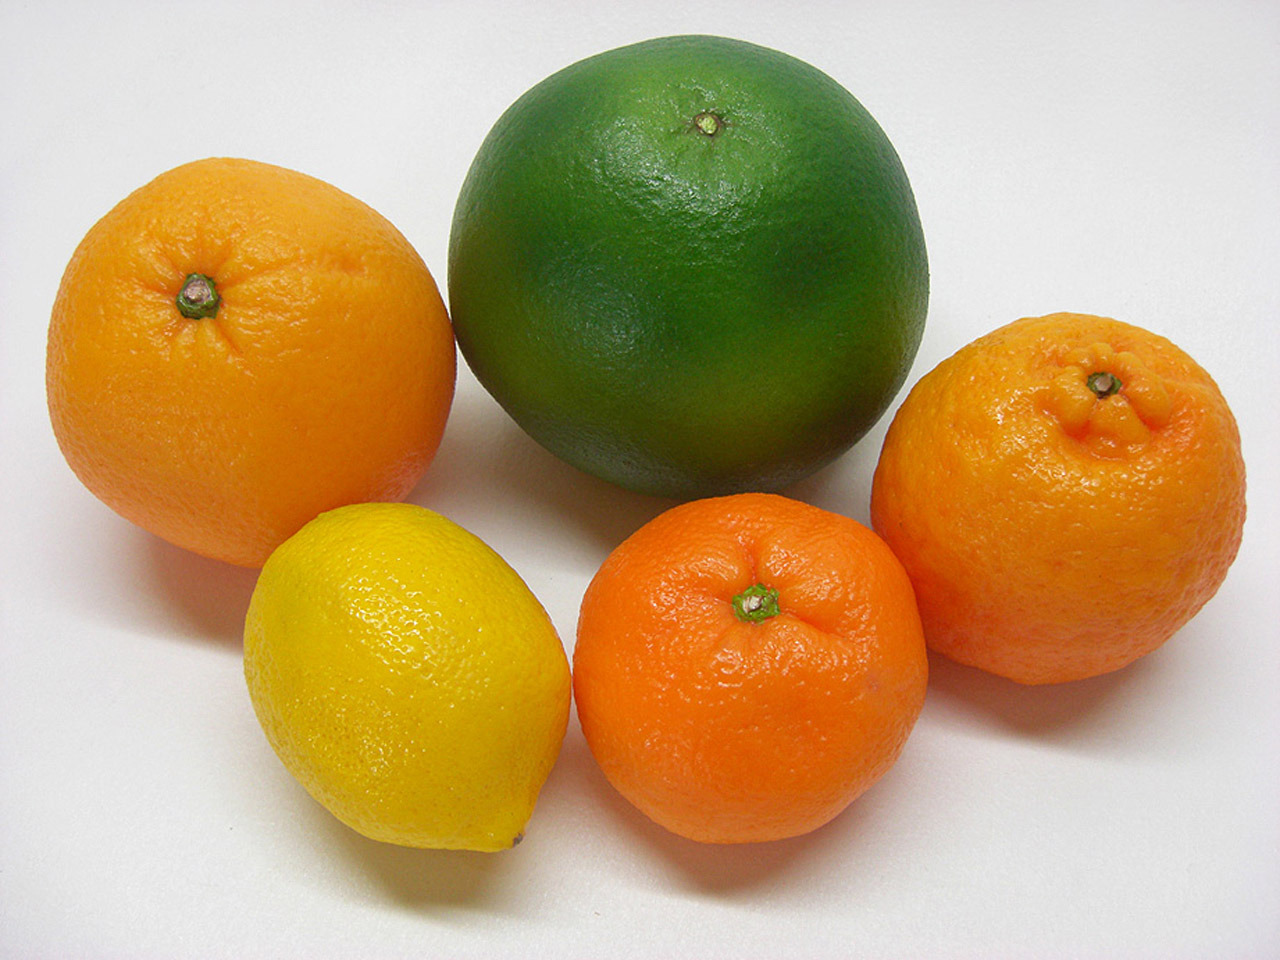
\includegraphics[width=0.8\textwidth]{images/image_3}
      \end{minipage}
      \begin{minipage}{0.4\textwidth}
        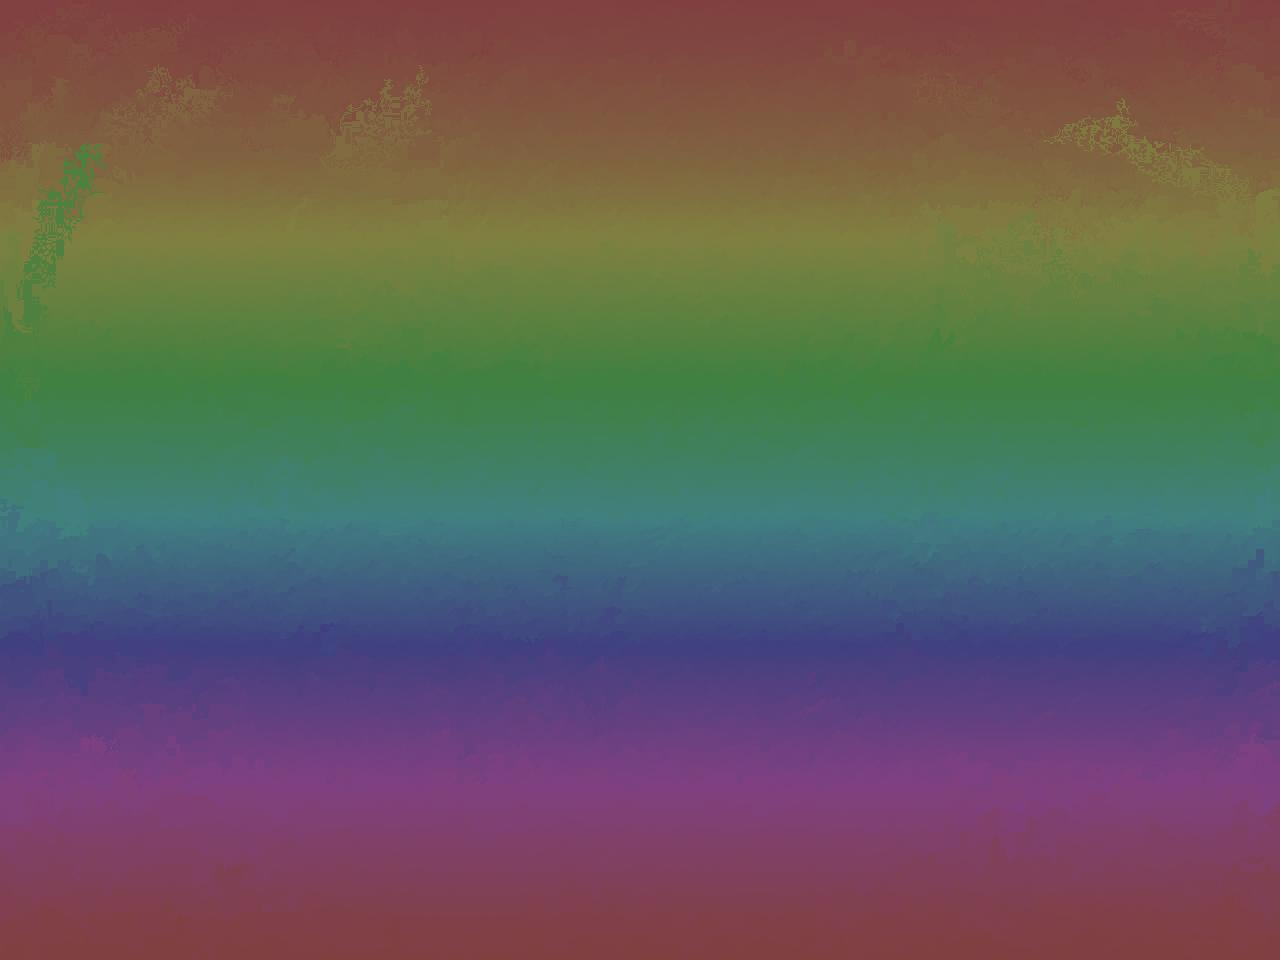
\includegraphics[width=0.8\textwidth]{images/result_image3}
      \end{minipage}
      \caption{A la izquierda la imágen 3, y la derecha el resultado de su segmentación. Esta tomó 4 horas en generarse.}
    \end{figure}

    \subsection{Resultados para imágenes buscadas}
      Debido a la limitación en el tamaño impuesta por la implementación poco eficiente, se utilizaron imágenes de baja resolución (256x256 pixéles).

      \begin{figure}[H]
        \centering
        \begin{minipage}{0.4\textwidth}
          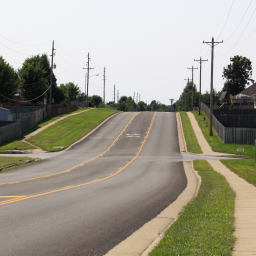
\includegraphics[width=0.8\textwidth]{images/image_6}
        \end{minipage}
        \begin{minipage}{0.4\textwidth}
          \includegraphics[width=0.8\textwidth]{images/result_image6}
        \end{minipage}
        \caption{A la izquierda la imágen 6, y la derecha el resultado de su segmentación. Esta tomó 13 minutos en generarse.}
      \end{figure}

      \begin{figure}[H]
        \centering
        \begin{minipage}{0.4\textwidth}
          \includegraphics[width=0.8\textwidth]{images/image_7}
        \end{minipage}
        \begin{minipage}{0.4\textwidth}
          \includegraphics[width=0.8\textwidth]{images/result_image7}
        \end{minipage}
        \caption{A la izquierda la imágen 7, y la derecha el resultado de su segmentación. Esta tomó 4 minutos en generarse.}
      \end{figure}

      \begin{figure}[H]
        \centering
        \begin{minipage}{0.4\textwidth}
          \includegraphics[width=0.8\textwidth]{images/image_8}
        \end{minipage}
        \begin{minipage}{0.4\textwidth}
          \includegraphics[width=0.8\textwidth]{images/result_image8}
        \end{minipage}
        \caption{A la izquierda la imágen 8, y la derecha el resultado de su segmentación. Esta tomó 5 minutos en generarse.}
      \end{figure}

      \begin{figure}[H]
        \centering
        \begin{minipage}{0.4\textwidth}
          \includegraphics[width=0.8\textwidth]{images/image_9}
        \end{minipage}
        \begin{minipage}{0.4\textwidth}
          \includegraphics[width=0.8\textwidth]{images/result_image9}
        \end{minipage}
        \caption{A la izquierda la imágen 9, y la derecha el resultado de su segmentación. Esta tomó 8 minutos en generarse.}
      \end{figure}

      \begin{figure}[H]
        \centering
        \begin{minipage}{0.4\textwidth}
          \includegraphics[width=0.8\textwidth]{images/image_10}
        \end{minipage}
        \begin{minipage}{0.4\textwidth}
          \includegraphics[width=0.8\textwidth]{images/result_image10}
        \end{minipage}
        \caption{A la izquierda la imágen 10, y la derecha el resultado de su segmentación. Esta tomó 8 minutos en generarse.}
      \end{figure}

  Todas las segmentaciones fueron calculadas en un computador corriendo Ubuntu 18.04, con 16gb de RAM y reloj de CPU a 3.2 GHz. 

\section{Conclusiones}
  El algoritmo propuesto para esta tarea era más costoso que los anteriores, por lo que la optimización era extremadamente importante. Debido a esto, al no conseguir una versión óptima, se hizo difícil el testeo de los resultados, lo que dificultó mucho el poder encontrar bugs en el funcionamiento y una posible razón de porqué el algoritmo entregaba segmentaciones tan malas.

  Una posible falta en el algoritmo implementada es la búsqueda del MST de un cluster. En la implementación actual estos se calculan cuando se necesitan para cada nodo. Esto implica conseguir la lista de todos los nodos en el cluster correspondiente, y para cada pixel buscar sus vecinos, ver si cada vecino pertenece al cluster usando Union-Find, y luego agregar el peso en el diccionario de pesos a una lista, la cual luego es ordenada por pesos no-crecientes y se comienza el algoritmo de Kruskal para encontrar el MST. Esto podría ser cambiado por tener pre-calculados los MST de cada cluster, y al haber una mezcla de clusters, sólo uniéndolos con la arista de menor peso que conecte a los dos cluster (la cual siempre será la arista que causó la unión). De este modo no se deben recalcular en todas las iteraciones, y se la mezcla de distintos MST es mucho más rápida. 

% FIN DEL DOCUMENTO
\end{document}
